\chapter{Phương pháp và Thiết kế hệ thống}
\label{chap:methodology}

Chương này trình bày chi tiết phương pháp luận thiết kế và toàn bộ kiến trúc của
hệ thống. Chúng tôi bắt đầu từ cái nhìn tổng thể về kiến trúc bốn thành phần và
mô hình Execute--Order--Validate, sau đó đặc tả mô hình dữ liệu chung, rồi đi
sâu vào thiết kế của từng thành phần theo đúng hành trình của một giao dịch:
Core Service (cổng vào và thực thi), Ordering Service (đồng thuận Raft ---
trọng tâm), Committing Peer (kiểm tra và ghi sổ), và Blockchain Explorer (giao
diện). Cuối chương trình bày cơ sở dữ liệu PostgreSQL và phương pháp đo lường
hiệu năng.

\section{Tổng quan kiến trúc}
\label{sec:architecture-overview}

\subsection{Triết lý thiết kế: tách ba trách nhiệm}

Hệ thống được tổ chức theo triết lý \textbf{Execute--Order--Validate} của
Hyperledger Fabric (đã giới thiệu ở Mục~\ref{sec:fabric}), trong đó ba trách
nhiệm cốt lõi của việc xử lý một giao dịch được tách thành ba tiến trình độc
lập:

\begin{table}[H]
\centering
\caption{Ba tầng trách nhiệm và ranh giới của chúng}
\label{tab:three-tiers}
\begin{tabular}{@{}p{2.6cm}p{3.4cm}p{3.6cm}p{3.2cm}@{}}
\toprule
\textbf{Tầng} & \textbf{Thành phần} & \textbf{Làm gì} & \textbf{Không làm gì} \\
\midrule
Execute & Core Service & Chạy hợp đồng, xin endorsement & Không quyết định thứ tự \\
Order & Ordering Service (Raft) & Quyết định thứ tự, gom block & Không chạy hợp đồng, không xét nội dung \\
Validate & Committing Peer & Kiểm tra \& ghi vĩnh viễn & Không sắp xếp lại thứ tự \\
\bottomrule
\end{tabular}
\end{table}

Việc tách tiến trình mang lại bốn lợi ích thực tiễn: (1)~\textbf{chịu lỗi} ---
Ordering Service gồm nhiều node, chết một node vẫn chạy nhờ Raft; (2)~\textbf{mở
rộng độc lập} --- cần thêm sức tính hợp đồng thì thêm Core Service, cần ghi
nhanh hơn thì thêm Committing Peer; (3)~\textbf{bảo mật theo lớp} --- mỗi tầng
chỉ thấy thông tin nó cần, ví dụ Ordering Service không cần biết nội dung giao
dịch; và (4)~\textbf{phản ánh đúng thực tế doanh nghiệp}, giống mô hình mà ngành
tài chính và chuỗi cung ứng đang dùng.

\subsection{Sơ đồ tổng thể}

Hệ thống gồm bốn thành phần chạy độc lập, giao tiếp với nhau qua mạng ngang hàng
\texttt{libp2p}, cùng một cơ sở dữ liệu PostgreSQL đóng vai trò bản sao tra cứu.
Hình~\ref{fig:overall-arch} mô tả kiến trúc và các luồng giao tiếp chính.

\begin{figure}[H]{}
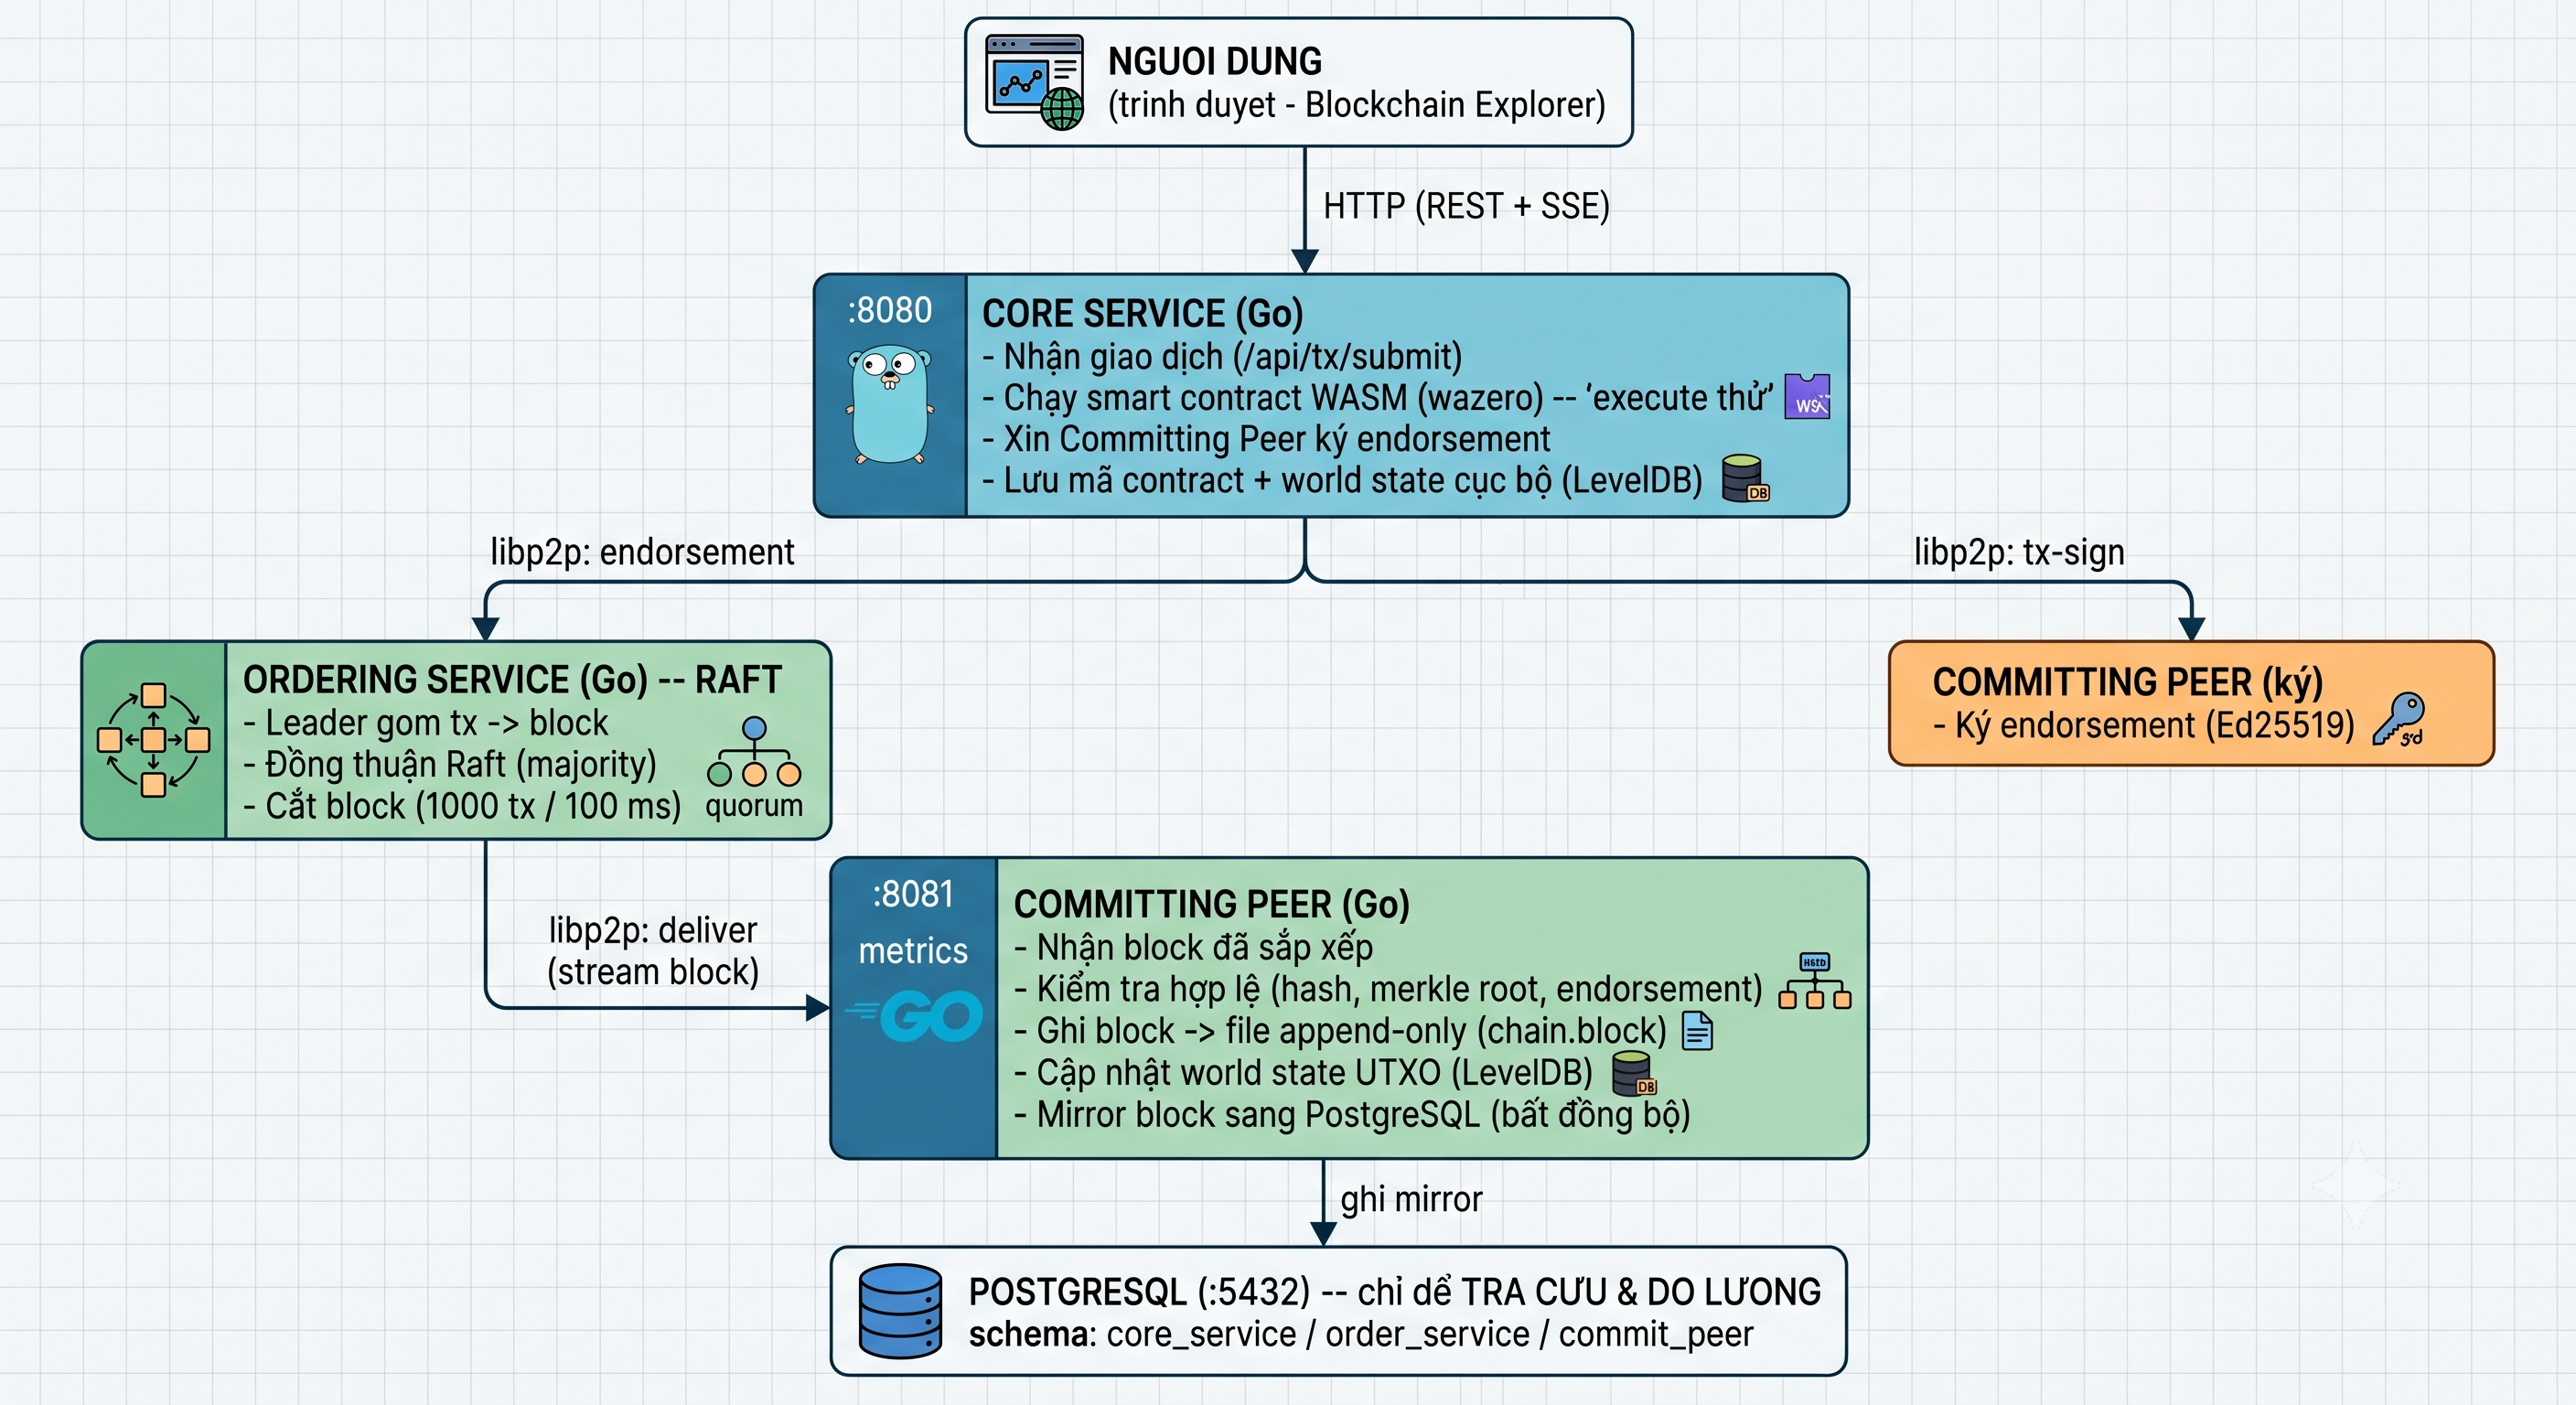
\includegraphics[width=\textwidth]{Images/fg_1_architecture.png}
\centering
\caption{Kiến trúc tổng thể và các luồng giao tiếp chính của hệ thống.}
\label{fig:overall-arch}
\end{figure}

\textbf{Một điểm thiết kế quan trọng:} PostgreSQL \textbf{không} nằm trong luồng
đồng thuận. Nó chỉ là bản sao (mirror) để Explorer tra cứu và để đo
throughput/latency. Sổ cái ``thật'' nằm ở file \texttt{chain.block} và LevelDB
của Committing Peer. Nếu PostgreSQL chết, blockchain vẫn chạy bình thường --- một
quyết định kiến trúc giúp tốc độ ghi sổ không bị phụ thuộc vào tốc độ của một cơ
sở dữ liệu ngoài.

\subsection{Hành trình của một giao dịch}
\label{sec:tx-journey}

Để hiểu cách các thành phần phối hợp, ta theo dõi hành trình end-to-end của một
giao dịch gọi hợp đồng \texttt{demo\_inventory} để đăng ký 100 sản phẩm:

\begin{enumerate}
  \item \textbf{Tạo \& gửi:} Người dùng điền form trên Explorer; frontend mã hóa
  dữ liệu thành payload nhị phân (hex) và gửi \texttt{POST /api/tx/submit} tới
  Core Service. Giao dịch gồm \texttt{txid}, \texttt{contract\_name},
  \texttt{function\_name}, \texttt{payload}.
  \item \textbf{Execute thử:} Core Service nạp WASM của hợp đồng, chạy hàm kiểm
  tra với payload. Thành công thì tiếp tục; thất bại trả lỗi ngay.
  \item \textbf{Xin endorsement:} Core mở stream \texttt{tx-sign} tới Committing
  Peer; peer ký Ed25519 và trả lại giao dịch kèm chữ ký xác nhận.
  \item \textbf{Gửi đi sắp xếp:} Core hỏi Discovery ai là Leader của cluster
  Raft, rồi gửi giao dịch (đã endorse) qua stream \texttt{endorsement} tới
  Leader; đồng thời ghi thời điểm gửi để đo latency.
  \item \textbf{Đồng thuận \& cắt block:} Leader gom giao dịch vào TxPool; khi
  đủ 1000 giao dịch \textit{hoặc} sau 100\,ms, cắt một block, tính hash + Merkle
  root, gửi đề xuất cho Follower. Khi đa số Follower ACK, Leader commit block.
  \item \textbf{Giao block:} Block vừa commit được phát tỏa (fan-out) qua stream
  \texttt{deliver} tới mọi Committing Peer.
  \item \textbf{Kiểm tra \& ghi:} Committing Peer kiểm tra hash, Merkle root,
  endorsement; nếu hợp lệ thì ghi block vào \texttt{chain.block} và cập nhật
  world state UTXO trong LevelDB (một thao tác ghi nguyên tử).
  \item \textbf{Mirror \& hiển thị:} Committing Peer ghi bản sao sang PostgreSQL
  bất đồng bộ; Core đọc lại và đẩy cập nhật về trình duyệt qua SSE để Explorer
  hiển thị gần như tức thì.
\end{enumerate}

\section{Mô hình dữ liệu}
\label{sec:data-model}

Trước khi đi vào từng thành phần, cần thống nhất các cấu trúc dữ liệu được dùng
xuyên suốt hệ thống.

\subsection{Giao dịch (Transaction)}

Hệ thống hỗ trợ \textbf{đồng thời hai mô hình} giao dịch: mô hình hợp đồng thông
minh (gọi hàm, ghi world state) và mô hình UTXO (Vin/Vout). Cấu trúc
\texttt{Transaction} (trong \texttt{coreservice/internal/core/model.go}) phản
ánh cả hai:

\begin{lstlisting}[language=Go,caption={Cấu trúc Transaction và Endorsement},captionpos=b]
type EndorsementEntry struct {
    PublicKey string   // khoa cong khai cua peer xac nhan
    Signature string   // chu ky
}

type Transaction struct {
    Txid         string
    ContractName string
    FunctionName string
    Payload      []byte             // nhi phan, JSON ma hoa hex
    Endorsements []EndorsementEntry // mang chu ky xac nhan
    Signature    string             // (legacy) phan chieu endorsement cuoi
    SenderPubKey string             // (legacy) khoa cua endorser cuoi
    Vin          []VIN              // ho tro UTXO: dau vao
    Vout         []VOUT             // ho tro UTXO: dau ra
    Version      uint32
    LockTime     uint32
}
\end{lstlisting}

Hai trường \texttt{Signature} và \texttt{SenderPubKey} là kiểu cũ (một chữ ký);
hệ thống mới ưu tiên mảng \texttt{Endorsements[]} để hỗ trợ \textit{nhiều} chữ
ký xác nhận. Khi serialize JSON, \texttt{Payload} được mã hóa hex thông qua các
hàm \texttt{MarshalJSON}/\texttt{UnmarshalJSON} tùy chỉnh, nhằm biểu diễn dữ
liệu nhị phân an toàn trong JSON.

\subsection{Block}

Một block tóm tắt một tập giao dịch đã được sắp xếp, với một header kiểu Bitcoin:

\begin{itemize}
  \item \texttt{Timestamp}: thời điểm tạo block.
  \item \texttt{PrevHash}: hash của block trước (nối chuỗi).
  \item \texttt{MerkleRoot}: gốc cây Merkle tính từ danh sách \texttt{txid}.
  \item \texttt{Nonce}: giá trị phụ trong header.
  \item \texttt{Hash}: double-SHA256 của header --- ``dấu vân tay'' của block.
  \item \texttt{Transactions}: danh sách giao dịch trong block.
\end{itemize}

Block hash được tính bằng \textbf{double-SHA256} của header (giống Bitcoin), và
phải được tính \textit{y hệt} ở cả ba thành phần sinh/kiểm tra block (Ordering
Service khi tạo, Committing Peer khi kiểm tra) để đảm bảo nhất quán.

\subsection{World State và mô hình UTXO}

\textbf{World state} là ảnh chụp trạng thái hiện tại của hệ thống, tính được từ
toàn bộ lịch sử block. Trong khi chuỗi block là lịch sử bất biến (chỉ thêm),
world state là bản đồ key$\rightarrow$value có thể ghi đè. Với mô hình UTXO,
world state là một \textit{tập các UTXO chưa tiêu}, với lược đồ key:
\[
\texttt{utxo:}\langle\texttt{txid}\rangle\texttt{:}\langle\texttt{vout\_index}\rangle
\;\longrightarrow\; \text{JSON của VOUT}
\]
Khi áp dụng một block, mỗi \texttt{VIN} sẽ \textit{xóa} một UTXO (đánh dấu đã
tiêu), mỗi \texttt{VOUT} sẽ \textit{tạo} một UTXO mới --- toàn bộ trong một thao
tác ghi nguyên tử (xem Mục~\ref{sec:cp-storage}).

\subsection{Log entry của Raft}

Ở tầng đồng thuận, mỗi đơn vị nhân bản là một \texttt{LogEntry} bao bọc một
block:

\begin{lstlisting}[language=Go,caption={Cấu trúc LogEntry trong Raft},captionpos=b]
type LogEntry struct {
    Index        int64   // vi tri trong log
    PrevLogIndex int64   // index cua entry lien truoc (kiem tra lien tuc)
    Term         int64   // term khi tao
    Type         string  // "BLOCK_PROPOSING"
    Block        Block   // block thuc su
}
\end{lstlisting}

Trường \texttt{PrevLogIndex} cho phép Follower kiểm tra log có \textbf{liên tục}
hay không (không bị nhảy cóc) trước khi chấp nhận entry mới --- đây là cốt lõi
đảm bảo an toàn của Raft.

\section{Core Service --- Cổng vào và Tầng tính toán}
\label{sec:core-service}

\subsection{Vai trò}

\textbf{Core Service} (\texttt{coreservice/}, viết bằng Go, cổng HTTP
\texttt{:8080}) là cổng vào và đồng thời là tầng tính toán của hệ thống, tương
ứng vai trò Endorsing Peer/Gateway trong Fabric. Mọi giao dịch của người dùng
đều đi qua đây đầu tiên. Ba nhiệm vụ chính: (1)~thực thi hợp đồng thông minh
WASM trong sandbox cô lập để ``chạy thử''; (2)~điều phối endorsement và gửi giao
dịch tới Leader của Ordering Service; (3)~phục vụ REST API, SSE realtime và tổng
hợp số liệu benchmark.

Core Service gần như \textit{không trạng thái} (stateless) đối với sổ cái:
trạng thái chốt cuối nằm ở Committing Peer; Core chỉ giữ bản cache cục bộ (mã
contract, world state demo) và đọc lại từ PostgreSQL khi cần hiển thị.

\subsection{Luồng khởi động}

Khi chạy (\texttt{cmd/node/main.go}), Core Service thực hiện tuần tự: (1)~dựng
libp2p host lắng nghe \texttt{/ip4/0.0.0.0/tcp/0}; (2)~kết nối PostgreSQL với
thử lại 10 lần --- nếu thất bại vẫn chạy ở chế độ hạn chế; (3)~mở hai instance
LevelDB (\texttt{contract\_db} và \texttt{ledger\_db}), thử lại 3 lần và xóa file
LOCK nếu kẹt; (4)~tạo \texttt{WasmEngine} với pool module; (5)~nhập địa chỉ
Orderer \& Committing Peer rồi làm ấm kết nối; (6)~đăng ký route HTTP và chạy
server; (7)~chờ tín hiệu dừng để tắt mượt.

\subsection{Máy ảo hợp đồng thông minh WASM}
\label{sec:wasm-engine}

Khi Core nhận \texttt{POST /api/tx/submit}, bước đầu tiên là \textbf{simulate} logic
hợp đồng trong \texttt{WasmEngine} (\texttt{internal/vm/engine.go}). Runtime dùng
\textbf{wazero} (Go-native, không cần CGO) kèm WASI
(\texttt{wasi\_snapshot\_preview1}). Bytecode đọc từ LevelDB
(\texttt{data/contract\_db}, key = \texttt{contract\_name}). Nếu contract từ chối
payload hoặc runtime lỗi, API trả HTTP 400 và dừng --- chưa ký endorsement, chưa
gửi orderer. Phần dưới mô tả ABI, vòng đời một lần \texttt{Execute}, cơ chế cache/pool,
quy trình biên dịch TinyGo, và ba contract mẫu.

\textbf{Kiến trúc runtime.} Mỗi Core node giữ \textbf{một} \texttt{wazero.Runtime} dùng
chung cho mọi contract. Lúc khởi tạo (\texttt{NewWasmEngine}): (i)~instantiate WASI
(cho \texttt{print}, file descriptor tối thiểu); (ii)~đăng ký host module
\texttt{env} export \texttt{PutState}; (iii)~tạo map \texttt{contractCache} và
\texttt{pools}. \texttt{StateDB} tách hai LevelDB: \texttt{contract\_db} (bytecode
WASM + metadata schema) và \texttt{ledger\_db} (key/value do \texttt{PutState} ghi
khi simulate). Đây là state \textbf{cục bộ Core}, khác world state UTXO trên
Committing Peer.

\textbf{Giao diện host--contract (ABI).} Contract TinyGo và host thống nhất qua
export/import WASM. Contract \textbf{xuất} (\texttt{//export}):
\texttt{allocate(uint32 size) $\rightarrow$ uint32} cấp buffer trong linear memory;
host ghi payload vào offset trả về. \texttt{verify\_tx(ptr, size) $\rightarrow$ uint32}
(hoặc \texttt{execute}) là entry point, trả \texttt{1}/\texttt{0}. Contract
\textbf{nhập} qua \texttt{//go:wasmimport env PutState}: host đọc
\texttt{keyPtr/keySize}, \texttt{valPtr/valSize} từ RAM sandbox, gọi
\texttt{StateDB.PutState}; trả \texttt{1} nếu ghi LevelDB OK, \texttt{0} nếu đọc
memory lỗi hoặc DB lỗi.

Trong contract, payload thường được đọc bằng \texttt{unsafe.Slice} trên con trỏ
\texttt{ptr} (pattern \texttt{example\_asset}, \texttt{bench\_ping}). Key/value
truyền sang \texttt{PutState} cũng là con trỏ offset trong linear memory --- host
không nhận chuỗi Go trực tiếp. Hình~\ref{fig:wasm-abi} tóm tắt thứ tự gọi.

\begin{figure}[H]
\centering
\caption{Giao diện hàm (ABI) giữa host và contract WASM.}
\label{fig:wasm-abi}
\end{figure}

\textbf{Luồng \texttt{Execute(ctx, tx)} từng bước.}

\textit{Bước A --- Nạp và biên dịch.} \texttt{getOrCompile(tx.ContractName)}:
đọc RLock \texttt{contractCache}; hit thì trả \texttt{CompiledModule} (warm).
Miss thì \texttt{GetContract} từ LevelDB, \texttt{CompileModule}, ghi cache dưới
Lock. Cold start gồm I/O đĩa + biên dịch WASM; warm chỉ còn phần instantiate (rẻ
hơn nhiều nhưng vẫn có chi phí nếu không có pool).

\textit{Bước B --- Lấy sandbox.} \texttt{acquireModule}: \texttt{poolFor} tạo pool
lần đầu gặp contract --- vòng lặp $N =$ \texttt{WASM\_POOL\_SIZE} lần
\texttt{InstantiateModule} (mặc định 16, max 32), đẩy vào channel có buffer $N$.
\texttt{select} non-blocking: có slot rảnh thì lấy ngay; không thì tạo instance
overflow (tên \texttt{contractName-<serial>}, serial tăng atomic). Mỗi instance
cấu hình \texttt{WithStartFunctions("\_initialize")} để TinyGo/WASI init chạy
trước khi gọi export.

\textit{Bước C --- Đưa payload vào sandbox.} Nếu \texttt{len(tx.Payload)>0}: gọi
\texttt{allocate(len)}, lấy \texttt{ptr} từ kết quả WASM, \texttt{Memory.Write}
copy byte payload (đã decode từ hex JSON ở tầng API). Thiếu export \texttt{allocate}
$\rightarrow$ lỗi ``thiếu hàm bắt buộc''. Payload rỗng vẫn gọi entry với
\texttt{ptr=0, size=0} (contract phải tự xử lý).

\textit{Bước D --- Gọi entry.} \texttt{FunctionName} từ tx, mặc định \texttt{execute}.
Engine thử danh sách fallback: nếu yêu cầu \texttt{execute} mà không có export thì
thử \texttt{verify\_tx}, và ngược lại --- tương thích contract cũ chỉ export một
tên. \texttt{Call(ctx, ptr, payloadLen)}; WASM trap/panic $\rightarrow$ lỗi runtime;
kết quả số \texttt{0} $\rightarrow$ lỗi nghiệp vụ (``bị Smart Contract từ chối'').

\textit{Bước E --- Trả sandbox.} \texttt{defer release(runOK)}: nếu thành công,
\texttt{runOK=true}, đẩy module lại channel; channel đầy thì \texttt{Close} instance
(thừa sandbox sau burst). Nếu lỗi, \texttt{runOK=false}, luôn \texttt{Close} ---
không recycle instance có thể ở trạng thái hỏng.

\textbf{Hai lớp tối ưu hiệu năng.}

\textit{(1) Compiled module cache} --- map in-memory theo tên contract, mutex
đọc/ghi. Một bytecode chỉ compile một lần cho đến khi restart Core. Phù hợp khi
cùng contract phục vụ hàng nghìn tx (benchmark \texttt{bench\_ping}).

\textit{(2) Module pool} --- channel \texttt{chan api.Module} giữ sẵn $N$ instance
đã link WASI + host \texttt{env}, tránh \texttt{InstantiateModule} lặp trên hot
path. Cho phép xử lý song song tối đa $N$ tx đồng thời trên cùng contract (mỗi
sandbox một linear memory riêng). Vượt $N$, engine vẫn phục vụ bằng instance tạm,
nhưng latency tăng và có thể đóng bỏ sau khi dùng.

\begin{table}[H]
\centering
\caption{Tham số và gỡ lỗi WASM engine}
\label{tab:wasm-env}
\begin{tabular}{@{}p{3.4cm}p{2.4cm}p{5.8cm}@{}}
\toprule
\textbf{Tham số} & \textbf{Mặc định} & \textbf{Ý nghĩa} \\
\midrule
\texttt{WASM\_POOL\_SIZE} & 16 (max 32) & Số sandbox giữ sẵn / contract \\
\texttt{CORE\_LOG} & tắt & \texttt{debug}: log cold/warm, WASM stdout/stderr \\
\bottomrule
\end{tabular}
\end{table}

\textbf{Biên dịch và triển khai contract.} Source nằm trong
\texttt{coreservice/contracts/<ten>/main.go}. Build:
\begin{lstlisting}[language=bash,numbers=none,caption={Bien dich WASM (TinyGo)},captionpos=b]
cd coreservice/contracts && ./build_wasm.sh
# hoac tung contract:
tinygo build -o my_contract.wasm -target wasi -no-debug -scheduler=none ./
\end{lstlisting}
\texttt{-target wasi}: link WASI snapshot mà wazero hỗ trợ. \texttt{-target wasm}
thuần (browser) kéo \texttt{gojs} --- host báo \texttt{module[gojs] not
instantiated}. \texttt{-scheduler=none}: không spawn goroutine scheduler TinyGo
trong module, giảm overhead và dễ lý giải trong sandbox. \texttt{-no-debug}: binary
nhỏ hơn. Output \texttt{my\_contract.wasm} deploy qua \texttt{POST /api/tx/deploy}
(multipart \texttt{contract\_name} + \texttt{file}) $\rightarrow$ lưu
\texttt{contract\_db} + tùy chọn \texttt{payload\_schema} JSONB trên Postgres.

\textbf{Payload trên wire.} Client (Explorer \texttt{Transfer}, k6) gửi
\texttt{payload} là \textbf{chuỗi hex} của JSON UTF-8. Core decode hex
$\rightarrow$ \texttt{[]byte} trong \texttt{Transaction.Payload} trước khi vào WASM.
Contract dùng \texttt{encoding/json} parse struct (ví dụ \texttt{\{id, color,
action\}}). \texttt{coercePayloadFieldsBySchema} phía frontend ép kiểu số trước
khi stringify để \texttt{json.Unmarshal} sang \texttt{int} không lỗi.

\textbf{Ba hợp đồng mẫu} (Bảng~\ref{tab:sample-contracts}).

\begin{table}[H]
\centering
\caption{Ba hợp đồng mẫu trong repository}
\label{tab:sample-contracts}
\begin{tabular}{@{}p{2.6cm}p{3.2cm}p{5.6cm}@{}}
\toprule
\textbf{Contract} & \textbf{Payload JSON} & \textbf{Logic chính} \\
\midrule
example\_asset & id, color, action & \texttt{action=="create"}: key \texttt{Asset\_<id>}, value = raw JSON payload, qua \texttt{PutState} \\
demo\_inventory & op, sku, qty & \texttt{op=="register"}, \texttt{qty>=0}: key \texttt{Inv\_<sku>} \\
bench\_ping & v (string) & \texttt{size<=512}, \texttt{1<=len(v)<=128}; validate only, \textbf{khong} \texttt{PutState} \\
\bottomrule
\end{tabular}
\end{table}

\texttt{bench\_ping} thiết kế cho benchmark throughput: không gọi host import, không
ghi LevelDB --- đo trần HTTP + WASM + ký + orderer. \texttt{example\_asset} minh
họa contract có side-effect: mọi trường hợp \texttt{action != "create"} hoặc
\texttt{PutState} trả \texttt{0} đều reject (\texttt{return 0}). Cả ba export
\texttt{allocate} + \texttt{verify\_tx}; engine resolve tên hàm tự động.

\textbf{Vị trí trong pipeline và giới hạn.} WASM simulate chạy \textbf{một lần}
tại Core trước endorsement. Committing Peer khi ghi block \textbf{không} gọi lại
\texttt{WasmEngine} --- chỉ kiểm tra endorsement, Merkle, hash. Do đó:
\texttt{PutState} trong simulate cập nhật \texttt{ledger\_db} Core (hữu ích demo/query
cục bộ) nhưng \textbf{chưa} đồng bộ tự động sang sổ cái commit peer; state contract
toàn mạng cần thiết kế thêm (ví dụ ghi state vào tx read-set/write-set, replay khi
commit). UTXO world state thật vẫn do commit peer \texttt{ApplyBlock} trên LevelDB
riêng. Tách bạch này quan trọng khi đọc kết quả Explorer: mirror Postgres phản
ánh tx đã commit, không phải mọi key \texttt{PutState} cục bộ trên Core.

\textbf{Tóm tắt chi phí theo pha.} Lần đầu deploy contract mới: compile + khởi tạo
pool ($N$ instantiate). Steady-state cùng contract: chỉ \texttt{allocate} +
\texttt{verify\_tx} + (tuỳ) \texttt{PutState} trên instance có sẵn --- đây là pha
engine tối ưu nhằm vào. Đổi \texttt{WASM\_POOL\_SIZE} khi benchmark nhiều client
song song: pool nhỏ $\rightarrow$ nhiều overflow/close; pool lớn (tới 32)
$\rightarrow$ RAM cao hơn nhưng ít instantiate đột biến.


\subsection{Mật mã và quá trình endorsement}
\label{sec:core-crypto}

Endorsement là lớp mật mã chứng minh một giao dịch smart-contract đã được ``chạy
thử'' hợp lệ trước khi vào ordering. Trong kiến trúc này, \textbf{Core Service
không tự ký} trên hot-path \texttt{POST /api/tx/submit}: sau
\texttt{engine.Execute()} (WASM), Core ủy quyền ký cho \textbf{Committing Peer}
qua libp2p, nhận tx đã có chữ ký, rồi chuyển tiếp orderer. Thuật toán ký
(\textbf{Ed25519} hoặc \textbf{ML-DSA-44}) được chọn \textbf{tại commit peer}
(\texttt{COMMIT\_PEER\_KEY\_ALGO}); Core giữ nguyên pipeline execute/relay và
đảm bảo trường \texttt{algorithm} không mất trên JSON wire.

\textbf{Hai scheme ký và vai trò từng tầng.}

\textit{Ed25519}~\cite{bernstein2012ed25519,rfc8032} (mặc định): chữ ký trên đường
cong Edwards, deterministic, khóa 32\,byte, chữ ký 64\,byte (128 ký tự hex trên
wire). Phù hợp benchmark throughput --- ký và serialize nhanh, response HTTP nhỏ.

\textit{ML-DSA-44} (FIPS\,204, post-quantum): triển khai trên commit peer qua
\texttt{cloudflare/circl/sign/mldsa/mldsa44}. Khóa công khai 1312\,byte (2624 hex),
chữ ký 2420\,byte (4840 hex). Core \textbf{không} gọi thư viện ML-DSA; chỉ thấy
payload JSON phình to sau bước tx-sign và khi relay sang orderer/block. Thời gian
\texttt{signTxViaCommitPeer()} tăng đáng kể so với Ed25519 --- nút thắt thường ở
ký post-quantum, không phải \texttt{engine.Execute()}.

Package \texttt{coreservice/internal/crypto} chỉ có helper \texttt{SignTransaction}/
\texttt{VerifyTransaction} Ed25519 (dev/legacy). Production luôn
\texttt{signTxViaCommitPeer()} $\rightarrow$ \texttt{Signer} pluggable trên commit
peer (\texttt{internal/crypto/signer.go}).

\begin{table}[H]
\centering
\caption{So sánh endorsement Ed25519 và ML-DSA-44 (góc nhìn Core)}
\label{tab:core-algo-compare}
\begin{tabular}{@{}lcc@{}}
\toprule
\textbf{Thuộc tính} & \textbf{Ed25519} & \textbf{ML-DSA-44} \\
\midrule
Cấu hình & \texttt{COMMIT\_PEER\_KEY\_ALGO=ed25519} & \texttt{mldsa-44} trên peer \\
Tên wire \texttt{algorithm} & \texttt{ed25519} & \texttt{mldsa-44} \\
Pubkey hex (điển hình) & 64 ký tự & 2624 ký tự \\
Chữ ký hex (điển hình) & 128 ký tự & 4840 ký tự \\
Ảnh hưởng Core execute & Không đổi & Không đổi \\
Ảnh hưởng tx-sign / HTTP & Nhẹ & Nặng (ký + JSON lớn) \\
\bottomrule
\end{tabular}
\end{table}

\textbf{Thông điệp ký và cấu trúc \texttt{EndorsementEntry}.} Message layout thống
nhất mọi tầng:
\begin{center}
\texttt{TxMessage = txid + contractName + string(payload)}
\end{center}
(\texttt{payload} là \texttt{[]byte} đã decode từ hex JSON). Mỗi endorsement:
\texttt{public\_key}, \texttt{signature}, \texttt{algorithm}. Struct trong
\texttt{internal/core/model.go}; serialize JSON với \texttt{payload} dạng hex.
Mảng \texttt{endorsements[]} là format chính; \texttt{sender\_pubkey}/
\texttt{signature} mirror entry cuối cho client cũ.

Khi commit peer ký, handler tx-sign gắn \texttt{algorithm} rõ ràng
(\texttt{ed25519} hoặc \texttt{mldsa-44}), self-verify trước khi trả Core. Core
merge vào tx rồi \texttt{json.Encode} gửi orderer; struct \texttt{Endorsement} bên
orderer cũng có field \texttt{algorithm} để block deliver tới commit peer không mất
metadata. Nếu \texttt{algorithm} thiếu (relay cũ), validator commit peer suy luận
từ độ dài hex (\texttt{InferAlgorithmFromWire}) --- tránh verify Ed25519 nhầm lên
chữ ký ML-DSA.

\textbf{Khóa tin cậy.} Commit peer validate block với
\texttt{TRUSTED\_ENDORSER\_PUBLIC\_KEYS}: danh sách \texttt{algo:pubhex} hoặc hex
thuần (mặc định hiểu Ed25519). Khi chạy ML-DSA, pubkey phải dạng
\texttt{mldsa-44:<hex>} --- không dùng pubkey Ed25519 cũ. Core không kiểm tra
chữ ký lúc submit; tin commit peer đã verify và chỉ ký khi self-check OK.

\textbf{Luồng \texttt{POST /api/tx/submit}.}

\begin{lstlisting}[numbers=left,caption={Luong xu ly submit (Core Service)},captionpos=b]
1. Decode JSON Transaction (payload hex -> []byte)
2. engine.Execute()              -> WASM simulate
       | fail -> HTTP 400
       v OK
3. signTxViaCommitPeer()         -> libp2p tx-sign
       |   peer: SignTx + EndorsementEntry{algorithm}
       |   fail -> HTTP 502
       v
4. sendEndorsementAsync()        -> orderer leader (libp2p)
5. SubmitRecorder.Record()       -> tx_submit_times (async)
6. HTTP 200 + signature preview + endorsement_count
\end{lstlisting}

\textit{Bước 1--2.} \texttt{submittedAt := time.Now()} ghi nhận sớm cho metric.
Decode body; \texttt{Execute(ctx, tx)} chạy WASM (mục~\ref{sec:wasm-engine}). Mọi
lỗi contract $\rightarrow$ HTTP 400, không ký.

\textit{Bước 3.} \texttt{signTxViaCommitPeer}: parse \texttt{COMMIT\_PEER\_P2P}
(comma-separated multiaddr), thử tuần tự. \texttt{SignTransactionViaCommitPeer}:
encode tx JSON $\rightarrow$ stream \texttt{/fabric-enterprise/commit-peer/tx-sign/1.0.0}
$\rightarrow$ decode \texttt{\{ok, error, tx\}}. \textbf{Sign pool}
(\texttt{CORE\_SIGN\_POOL}, mặc định bật): giữ TCP/libp2p ấm, mỗi request vẫn mở
stream mới (một round-trip), timeout \texttt{CORE\_SIGN\_TIMEOUT} (15\,s). Tx trả
về đã có \texttt{endorsements[0]} với \texttt{algorithm} khớp scheme peer đang
chạy. Với ML-DSA, response body có thể ~8--10\,KB/tx chỉ riêng phần chữ ký --- ảnh
hưởng bandwidth k6/Explorer nhưng không đổi logic API.

\textit{Bước 4.} \texttt{sendEndorsementAsync}: nếu có orderer discovery,
\texttt{discovery.SendEndorsement} gửi tx JSON (đã endorse) tới Raft leader qua
\texttt{/raft-order-service/endorsement/1.0.0}. Mặc định \texttt{CORE\_ASYNC\_ENDORSE=1}:
goroutine nền, HTTP 200 ngay sau bước 3. \texttt{CORE\_ENDORSE\_FALLBACK=1}: thử
follower nếu leader từ chối. Lỗi gửi orderer \textbf{không} đổi HTTP response (đã
200) --- tx có thể kẹt nếu async fail; benchmark cần theo dõi log orderer.

\textit{Bước 5.} \texttt{SubmitRecorder}: channel buffer 65536, worker flush batch
512 dòng / 50\,ms vào \texttt{core\_service.tx\_submit\_times}
(\texttt{ON CONFLICT DO NOTHING}). Tắt bằng \texttt{CORE\_RECORD\_SUBMIT=0}. Queue
đầy thì drop --- ưu tiên không chặn submit. Dùng join E2E với
\texttt{committed\_at} (mirror hoặc API commit peer \texttt{:8081}).

\textbf{Execute--Order--Validate trên Core.} Core = simulate + delegate sign +
forward. Orderer không verify chữ ký endorsement (để commit peer làm). Commit peer
khi ghi block gọi \texttt{VerifyEndorsement(txMessage, algorithm, sig, pub)} và
so \texttt{algo:pubhex} với trusted set. Tx gian lận (execute lợi dụng lỗ hổng
không có trong thiết kế hiện tại) vẫn cần endorsement hợp lệ từ khóa tin cậy ---
thiếu hoặc sai algorithm/sig $\rightarrow$ \texttt{block rejected}.

\textbf{Chuyển đổi scheme khi benchmark.} So sánh Ed25519 vs ML-DSA trên cùng Core:
(i)~restart commit peer với \texttt{COMMIT\_PEER\_KEY\_ALGO} và file khóa tương ứng
(\texttt{endorsement.key} / \texttt{endorsement.mldsa44.key}); (ii)~cập nhật
\texttt{TRUSTED\_ENDORSER\_PUBLIC\_KEYS}; (iii)~không đổi Core/WASM/k6 contract.
\texttt{engine.Execute()} và \texttt{TxMessage} giữ nguyên --- chỉ bước 3--4 và
kích thước JSON thay đổi. Metric E2E vẫn hợp lệ vì \texttt{RecordBlock} commit peer
không phụ thuộc algorithm.

\begin{table}[H]
\centering
\caption{Biến môi trường endorsement trên Core Service}
\label{tab:core-endorse-env}
\begin{tabular}{@{}p{3.6cm}p{2.2cm}p{5.8cm}@{}}
\toprule
\textbf{Biến} & \textbf{Mặc định} & \textbf{Tác dụng} \\
\midrule
\texttt{COMMIT\_PEER\_P2P} & (bắt buộc) & Multiaddr peer ký; nhiều addr cách nhau dấu phẩy \\
\texttt{CORE\_ASYNC\_ENDORSE} & \texttt{1} & Gửi orderer nền sau khi ký \\
\texttt{CORE\_ENDORSE\_FALLBACK} & tắt & \texttt{1}: dial follower khi leader lỗi \\
\texttt{CORE\_SIGN\_POOL} & bật & Kết nối libp2p ấm tới commit peer \\
\texttt{CORE\_SIGN\_TIMEOUT} & \texttt{15s} & Timeout mỗi lần tx-sign \\
\texttt{CORE\_RECORD\_SUBMIT} & bật & Ghi \texttt{tx\_submit\_times} (benchmark E2E) \\
\bottomrule
\end{tabular}
\end{table}

Biến thuật toán (\texttt{COMMIT\_PEER\_KEY\_ALGO}, \texttt{TRUSTED\_ENDORSER\_PUBLIC\_KEYS})
cấu hình trên \textbf{commit peer}, không trên Core --- Core chỉ cần
\texttt{COMMIT\_PEER\_P2P} trỏ đúng peer đang chạy scheme mong muốn.


\subsection{Mạng libp2p và Discovery}
\label{sec:core-network}

Mọi giao tiếp của Core với orderer và committing peer đều qua \textbf{stream}
libp2p, phân loại bằng Protocol ID (xem Bảng~\ref{tab:protocols}). Hai cơ chế
quan trọng cho hiệu năng và độ tin cậy:

\textbf{Connection pool ấm:} mở kết nối mới mỗi lần ký rất tốn (bắt tay TCP +
libp2p). Core giữ sẵn một \textit{kết nối ấm} tới Committing Peer
(\texttt{CORE\_SIGN\_POOL}, mặc định bật); mỗi lần ký chỉ mở một \textit{stream}
mới trên kết nối sẵn có, rẻ hơn nhiều. Có cơ chế thử lại 2 lần và tự kết nối
lại nếu hỏng.

\textbf{Discovery --- tìm Leader:} Ordering Service có nhiều node và Leader có
thể đổi. \texttt{Discovery Client} khởi tạo với danh sách bootstrap (vài
multiaddr orderer), gọi \texttt{Refresh()} để lấy \textit{membership view}
(danh sách thành viên + ai là Leader) và cache lại (TTL ${\sim}8$ giây). Khi
phát hiện Leader cũ lỗi, \texttt{Invalidate()} xóa cache nóng và tạm dùng bản
tốt cuối (\texttt{lastGood}) trong cửa sổ failover ${\sim}2$ phút. Cơ chế cache
+ failover này giúp Core chịu được việc Leader đổi mà không cần khởi động lại.

\subsection{Lưu trữ}

Core dùng hai loại lưu trữ. \textbf{LevelDB} (nhúng cục bộ) mở hai instance:
\texttt{ContractDB} lưu bytecode WASM và schema UI của contract, \texttt{LedgerDB}
lưu world state demo. \textbf{PostgreSQL} là bản sao chỉ-đọc của sổ cái Committing
Peer, phục vụ hiển thị Explorer, lưu danh mục contract và đo benchmark.

Một chi tiết tối ưu đáng chú ý là \texttt{SubmitRecorder}
(\texttt{storage/submit\_recorder.go}): để đo E2E latency cần ghi thời điểm
submit của từng giao dịch, nhưng gọi DB cho \textit{mỗi} giao dịch ở 5000 TPS sẽ
làm sập DB. Giải pháp là \textbf{batch INSERT qua channel}: mỗi giao dịch chấp
nhận đẩy \texttt{(txid, submitted\_at)} vào một channel đệm lớn (${\sim}65$k);
một goroutine nền gom nhiều bản ghi rồi \texttt{INSERT} hàng loạt hoặc xả định
kỳ. Đây là mẫu \textit{batching} kinh điển để giảm số lần gọi I/O.

\subsection{REST API và realtime}

Core mở HTTP server tại \texttt{:8080} với các nhóm endpoint chính trong
Bảng~\ref{tab:core-api}.

\begin{table}[H]
\centering
\caption{Các endpoint chính của Core Service}
\label{tab:core-api}
\begin{tabular}{@{}p{4.6cm}p{1.6cm}p{5.2cm}@{}}
\toprule
\textbf{Route} & \textbf{Method} & \textbf{Mục đích} \\
\midrule
/api/tx/deploy & POST & Tải lên contract WASM (multipart) \\
/api/tx/submit & POST & Gửi giao dịch: chạy $\rightarrow$ ký $\rightarrow$ sắp xếp \\
/api/contracts & GET & Liệt kê contract đã deploy \\
/api/blocks & GET & Liệt kê block đã commit \\
/api/transactions & GET & Liệt kê giao dịch đã commit \\
/api/explorer/stream & GET (SSE) & Đẩy block/giao dịch mới realtime \\
/api/metrics/benchmark & GET & Tổng hợp submit + commit + E2E latency \\
/api/metrics/throughput & GET & Tốc độ commit theo cửa sổ \\
\bottomrule
\end{tabular}
\end{table}

Endpoint \texttt{/api/explorer/stream} dùng \textbf{Server-Sent Events (SSE)} ---
server đẩy dữ liệu một chiều xuống trình duyệt qua một kết nối HTTP giữ mở. Khi
có block/giao dịch mới, Core gửi sự kiện \texttt{ledger\_update}. SSE được chọn
thay WebSocket vì luồng dữ liệu ở đây một chiều (server$\rightarrow$client), SSE
đơn giản hơn và tự kết nối lại.

\section{Ordering Service --- Đồng thuận Raft}
\label{sec:ordering-service}

Ordering Service là thành phần trọng tâm của khóa luận cả về mặt kỹ thuật lẫn học
thuật. Đây là nơi hệ thống hiện thực một cơ chế \textbf{đồng thuận phân tán} theo
tinh thần Raft~\cite{ongaro2014raft} nhưng \textbf{tự viết hoàn toàn} bằng Go
(không dùng thư viện \texttt{etcd/raft} hay \texttt{hashicorp/raft}), với một biến
thể bầu lãnh đạo \textit{theo độ ưu tiên} thay cho bầu cử theo timeout ngẫu nhiên
của Raft nguyên bản. Mục này trình bày lần lượt: (i)~vai trò và bài toán tổng sắp
thứ tự; (ii)~kiến trúc và các thành phần bên trong một node; (iii)~mô hình thông
điệp và cách định tuyến; (iv)~vòng đời trạng thái của một node; (v)~quản lý thành
viên và độ ưu tiên; (vi)~cơ chế quá bán (quorum) và cách nó chống phân ly não
(split-brain); (vii)~quy trình bầu lãnh đạo chi tiết; (viii)~nhân bản log và cắt
block --- đường nóng quyết định throughput; (ix)~giao block cho tầng ghi sổ;
(x)~đồng bộ (sync) khi một node tụt hậu; (xi)~tầng mạng; và (xii)~các đánh đổi
thiết kế.

\subsection{Vai trò và bài toán tổng sắp thứ tự}
\label{sec:ordering-role}

Trong một hệ phân tán, nhiều giao dịch đến gần như đồng thời từ nhiều nguồn khác
nhau (nhiều Core Service, nhiều client). Nếu để mỗi bản sao sổ cái tự quyết định
thứ tự áp dụng các giao dịch đó, các bản sao sẽ nhanh chóng phân kỳ: cùng một tập
giao dịch nhưng áp dụng theo thứ tự khác nhau có thể dẫn tới trạng thái cuối cùng
khác nhau (đặc biệt với mô hình UTXO, nơi một đầu vào chỉ được tiêu đúng một lần).
Nhiệm vụ của Ordering Service là bảo đảm \textbf{mọi node trung thực đều quan sát
thấy cùng một chuỗi giao dịch theo đúng một thứ tự duy nhất} --- thuộc tính này
gọi là \textit{tổng sắp thứ tự} (total order). Đây là điều kiện tiên quyết để
world state hội tụ giống hệt nhau tại mọi Committing Peer.

Điểm quan trọng về ranh giới trách nhiệm: Ordering Service \textbf{không} thực thi
hợp đồng thông minh, \textbf{không} kiểm tra nội dung nghiệp vụ của giao dịch, và
\textbf{không} xác minh chữ ký endorsement. Nó chỉ nhận các giao dịch đã được Core
Service ``chạy thử'' và được Committing Peer ký xác nhận, rồi \textit{gom chúng vào
các block theo một thứ tự nhất quán} và phân phát các block đó. Việc kiểm tra hợp
lệ mật mã được ủy thác cho Committing Peer (Mục~\ref{sec:committing-peer}). Cách
phân tách này giữ cho đường nóng đồng thuận nhẹ và nhanh: chi phí trên mỗi giao
dịch tại tầng ordering gần như chỉ là chi phí xếp hàng và nhân bản, không kèm chi
phí tính toán hợp đồng hay mật mã.

Sổ cái mà Ordering Service duy trì hoàn toàn nằm trong bộ nhớ (RAM): một chuỗi các
block đã commit và một nhật ký (log) các entry chưa commit. Đây là một lựa chọn
thiết kế có chủ đích, ưu tiên tốc độ; hệ quả và cách bù đắp (cơ chế sync khi node
khởi động lại) được bàn ở Mục~\ref{sec:ordering-tradeoffs}.

\subsection{Kiến trúc và các thành phần bên trong một node}
\label{sec:ordering-components}

Mỗi node của Ordering Service là một tiến trình Go độc lập, được mô hình hóa bằng
một cấu trúc trung tâm gọi là \texttt{RaftNode}. Toàn bộ trạng thái đồng thuận của
node được gói trong cấu trúc này, và mọi luồng xử lý (goroutine) đều thao tác trên
đó dưới sự bảo vệ của một số khóa (mutex) được phân tách theo chức năng để giảm
tranh chấp. Bảng~\ref{tab:raft-components} liệt kê các thành phần chính bên trong
một node cùng vai trò của chúng.

\begin{table}[H]
\centering
\caption{Các thành phần bên trong một node của Ordering Service}
\label{tab:raft-components}
\begin{tabular}{@{}p{3.5cm}p{9.3cm}@{}}
\toprule
\textbf{Thành phần} & \textbf{Vai trò} \\
\midrule
Trạng thái đồng thuận & Trạng thái node (Follower/Leader/\dots), \textit{term} hiện tại, ID của Leader đang biết. Được bảo vệ bởi một khóa đọc--ghi chung. \\
Membership view & Bản đồ toàn bộ thành viên đã biết của cluster (sống và chết), kèm thời điểm tham gia, độ ưu tiên và cờ sống/chết; có một số phiên bản (version) để phát hiện thay đổi. \\
TxPool & Hồ chứa trong RAM các giao dịch đang chờ đóng block; chỉ Leader dùng. Được bảo vệ bằng khóa riêng để không tranh chấp với luồng đồng thuận. \\
RaftLog & Nhật ký các entry \textit{chưa} commit; mỗi entry bao một block cùng chỉ số vị trí (index), chỉ số của entry liền trước và \textit{term}. \\
OrderingBlock & Chuỗi các block \textit{đã} commit --- phần sổ cái mà node đã chốt. \\
Deliver Manager & Quản lý danh sách người đăng ký (các Committing Peer) và phát tỏa mỗi block mới commit tới họ. \\
Sync coordinator & Điều phối việc ``đuổi kịp'' khi node thiếu block (mới tham gia hoặc vừa hồi sinh). \\
Transport & Tầng vận chuyển bọc một host libp2p: mở/nhận stream, gửi và phát tỏa thông điệp. \\
Các kênh (channel) & Hàng đợi nội bộ nối các luồng: kênh thông điệp chung, kênh ACK block, kênh ACK bầu cử, kênh phản hồi trạng thái sync\dots \\
\bottomrule
\end{tabular}
\end{table}

\textbf{Mô hình đồng thời.} Khi khởi động, node chạy song song một số goroutine
thường trực: (1)~một \textit{bộ xử lý thông điệp} rút thông điệp từ kênh chung và
điều phối tới hàm xử lý tương ứng; (2)~một \textit{bộ giám sát heartbeat} chạy
theo nhịp cố định (mỗi giây) để phát hiện Leader mất tích hoặc để tự gửi heartbeat
nếu mình là Leader; và (3)~các handler stream do libp2p gọi mỗi khi có kết nối
đến (thông điệp đồng thuận, giao dịch từ Core, yêu cầu giao block, yêu cầu sync).
Ngoài ra, khi trở thành Leader, node còn chạy thêm một \textit{vòng cắt block tự
động}. Các luồng này phối hợp qua kênh và mutex, được thiết kế để đường nóng
(nhận giao dịch, cắt block, commit) không bị chặn bởi các luồng chậm.

\textbf{Phân tách khóa.} Một điểm đáng lưu ý về hiệu năng là việc tách các mutex
theo trách nhiệm: khóa trạng thái đồng thuận, khóa TxPool, khóa membership, khóa
sync và khóa vòng cắt block là độc lập nhau. Nhờ đó, việc Leader thêm giao dịch
vào TxPool (rất thường xuyên dưới tải cao) không tranh chấp với việc đọc/ghi trạng
thái term hay với luồng bầu cử. Đây là nền tảng để hệ thống duy trì throughput cao
mà vẫn an toàn về mặt đồng thời.

\subsection{Mô hình thông điệp và định tuyến}
\label{sec:ordering-messages}

Các node giao tiếp với nhau bằng một kiểu thông điệp thống nhất, gồm: loại thông
điệp, \textit{term} của người gửi, ID người gửi, phần dữ liệu kèm theo (tùy loại)
và nhãn thời gian. Bảng~\ref{tab:raft-messages} liệt kê các loại thông điệp và
mục đích của chúng, nhóm theo chức năng.

\begin{table}[H]
\centering
\caption{Các loại thông điệp của tầng đồng thuận}
\label{tab:raft-messages}
\begin{tabular}{@{}p{2.2cm}p{4.3cm}p{6.3cm}@{}}
\toprule
\textbf{Nhóm} & \textbf{Thông điệp} & \textbf{Mục đích} \\
\midrule
Heartbeat & Heartbeat & Leader báo ``tôi còn sống'' cho các Follower. \\
          & HeartbeatResponse & Follower báo lại cho một Leader ``ôi'' (stale) biết term/Leader hiện hành để nó tự thoái vị. \\
\midrule
Bầu cử & IAmNewLeader & Node ưu tiên cao nhất tuyên bố ``tôi là Leader mới'' cho toàn cluster. \\
       & LeaderClaimAck & Follower trả lời CHẤP NHẬN/TỪ CHỐI lời tuyên bố đó. \\
\midrule
Thành viên & MembershipUpdate & Yêu cầu gia nhập (từ node mới) hoặc phát tỏa toàn bộ danh sách thành viên (từ Leader). \\
           & MembershipAck & Leader xác nhận đã kết nạp và gửi kèm ảnh chụp thành viên. \\
           & MembershipRequest/Response & Truy vấn/đáp danh sách thành viên (chỉ đọc), dùng khi tìm Leader lúc gia nhập. \\
\midrule
Giao dịch & TxRequest/TxResponse & Chuyển tiếp giao dịch tới Leader và xác nhận đã nhận. \\
\midrule
Block & BlockProposal & Leader đề xuất một entry log (một block) tới các Follower. \\
      & BlockProposalAck & Follower báo đã chấp nhận (hoặc từ chối) đề xuất. \\
      & BlockCommit & Leader thông báo một block đã đạt quá bán và được commit. \\
\midrule
Đồng bộ & SyncStatusRequest/Response & Dò trạng thái commit của các peer để chọn nguồn ``đuổi kịp''. \\
\bottomrule
\end{tabular}
\end{table}

\textbf{Định tuyến hai tốc độ.} Điểm thiết kế đáng chú ý ở tầng định tuyến là
không phải mọi thông điệp đều đi qua cùng một hàng đợi. Đa số thông điệp (heartbeat,
bầu cử, thành viên, đồng bộ) được đẩy vào một \textit{kênh chung} và xử lý tuần tự
bởi bộ xử lý thông điệp. Tuy nhiên, hai loại thông điệp có tần suất cực cao trên
đường nóng --- \textit{giao dịch đến} và \textit{ACK đề xuất block} --- được tách
ra xử lý riêng ngay tại handler stream: giao dịch được nạp thẳng vào TxPool (mỗi
stream vốn đã chạy trong goroutine riêng), còn ACK block được đưa vào một kênh
chuyên dụng. Lý do là: dưới tải hàng nghìn giao dịch mỗi giây, nếu để mọi thứ dồn
vào một hàng đợi chung thì các thông điệp điều phối quan trọng (ACK, commit,
heartbeat) sẽ bị kẹt sau một hàng dài giao dịch (hiện tượng nghẽn đầu hàng ---
head-of-line blocking), làm chậm cả cụm. Việc tách kênh giữ cho tín hiệu đồng
thuận luôn thông suốt bất kể lưu lượng giao dịch.

\subsection{Vòng đời và các trạng thái của node}
\label{sec:ordering-states}

Mỗi node luôn ở một trong bốn trạng thái. So với Raft nguyên bản (Follower /
Candidate / Leader), thiết kế này thay \textit{Candidate} bằng
\texttt{ClaimingLeader} và bổ sung \texttt{Syncing}:

\begin{itemize}
  \item \textbf{Follower:} trạng thái mặc định. Node nghe heartbeat từ Leader,
  nhận và ACK các đề xuất block, đồng thời chuyển tiếp giao dịch mà nó nhận được
  tới Leader.
  \item \textbf{ClaimingLeader:} node ưu tiên cao nhất còn sống đang tự tuyên bố
  làm Leader và chờ thu đủ quá bán số phiếu chấp nhận.
  \item \textbf{Leader:} node đã được chọn; nó gom giao dịch, cắt block, điều phối
  commit, gửi heartbeat và phục vụ giao block cho tầng ghi sổ.
  \item \textbf{Syncing:} node đang kéo các block/entry còn thiếu từ các peer khác
  để đuổi kịp trạng thái cluster; trong thời gian này nó tạm hoãn xử lý đề xuất và
  commit để tránh làm việc trùng.
\end{itemize}

Hình~\ref{fig:raft-states} minh họa các phép chuyển trạng thái. Các phép chuyển
chính gồm: Follower~$\rightarrow$~ClaimingLeader khi phát hiện Leader hết hạn
heartbeat và chính mình là ứng viên ưu tiên cao nhất;
ClaimingLeader~$\rightarrow$~Leader khi thu đủ quá bán phiếu chấp nhận;
ClaimingLeader~$\rightarrow$~Follower khi hết thời gian mà không đủ phiếu;
Leader~$\rightarrow$~Follower khi nhận được bằng chứng có một Leader ở term cao
hơn (qua heartbeat hoặc qua phản hồi heartbeat); và bất kỳ trạng thái nào cũng có
thể chuyển sang Syncing khi phát hiện mình thiếu dữ liệu (mới gia nhập, hồi sinh
sau mất kết nối, hoặc nhận commit cho một block chưa có trong log).

\begin{figure}[H]
\centering
\caption{Sơ đồ chuyển trạng thái của một node trong Ordering Service.}
\label{fig:raft-states}
\end{figure}

\subsection{Quản lý thành viên và độ ưu tiên}
\label{sec:ordering-membership}

Mỗi node duy trì cục bộ một \textit{membership view} --- bản đồ toàn bộ thành viên
cluster mà nó biết. Với mỗi thành viên, view lưu: ID của peer, thời điểm tham gia,
một số \textbf{độ ưu tiên} (priority) và cờ sống/chết. Ngoài ra view có một số
\textbf{phiên bản} (version) tăng dần mỗi khi có thay đổi (kết nạp thành viên, đánh
dấu sống/chết), dùng để so sánh xem view của ai mới hơn.

\textbf{Độ ưu tiên gán theo thứ tự tham gia.} Khi một node được kết nạp, nó nhận
độ ưu tiên bằng số thành viên hiện có tại thời điểm đó. Nghĩa là node đầu tiên có
độ ưu tiên 0 (cao nhất), node thứ hai có độ ưu tiên 1, và cứ thế. \textbf{Tham gia
càng sớm thì số ưu tiên càng nhỏ, và số càng nhỏ thì mức ưu tiên càng cao.} Ứng
viên Leader hợp lệ tại mọi thời điểm chính là \textit{node còn sống có độ ưu tiên
nhỏ nhất}. Đây là điểm khác biệt cốt lõi so với Raft nguyên bản và là nền tảng cho
cơ chế bầu cử xác định ở Mục~\ref{sec:leader-election}.

\textbf{Luồng kết nạp.} Chỉ Leader mới có quyền kết nạp thành viên mới. Khi nhận
được yêu cầu gia nhập, Leader thêm node vào view của mình, phát tỏa toàn bộ view
mới cho mọi thành viên, rồi gửi riêng cho node mới một xác nhận kèm ảnh chụp view.
Nhờ Leader là điểm tuần tự hóa duy nhất cho các thay đổi thành viên, mọi node cuối
cùng hội tụ về cùng một danh sách với cùng cách gán độ ưu tiên.

\textbf{Đánh dấu chết.} Một thành viên bị đánh dấu chết trong hai tình huống:
Leader phát hiện không gửi được thông điệp tới một Follower (khi phát tỏa hoặc gửi
heartbeat) thì đánh dấu Follower đó chết và phát tỏa view cập nhật; hoặc một
Follower phát hiện Leader hết hạn heartbeat thì đánh dấu Leader chết trước khi khởi
động bầu cử. Điểm tinh tế là một thành viên bị đánh dấu chết \textbf{không} bị xóa
khỏi view --- nó vẫn được tính vào tổng số thành viên. Lý do liên quan trực tiếp
đến cơ chế quá bán chống split-brain, trình bày ngay dưới đây.

\subsection{Quá bán tính trên tổng số thành viên}
\label{sec:quorum}

Một quyết định an toàn then chốt của thiết kế là: ngưỡng \textbf{quá bán} (quorum)
được tính trên \textbf{tổng số thành viên đã biết} (cả node sống lẫn node đã bị
đánh dấu chết), chứ không phải chỉ trên số node đang sống. Cụ thể, nếu tổng số
thành viên là $N$ thì ngưỡng quá bán là
\[
  \text{quá bán} = \left\lfloor \tfrac{N}{2} \right\rfloor + 1 .
\]
Ngưỡng này được áp dụng ở hai nơi quan trọng nhất: khi một node tuyên bố làm Leader
(cần thu đủ quá bán phiếu chấp nhận), và khi Leader commit một block (cần đủ quá
bán ACK).

\textbf{Vì sao tính trên tổng chứ không trên số sống?} Đây chính là lá chắn nền
tảng chống \textbf{phân ly não} (split-brain). Giả sử một cluster năm node bị chia
đôi do sự cố mạng thành hai phân vùng, một bên ba node và một bên hai node. Nếu
quá bán được tính theo số node \textit{sống mà mỗi bên quan sát được}, thì bên nào
cũng có thể tự cho mình là ``đa số'' trong tầm nhìn hạn hẹp của nó và bầu ra một
Leader riêng --- kết quả là hai Leader cùng commit các block khác nhau, sổ cái
phân kỳ không thể hòa giải. Ngược lại, khi quá bán luôn tính trên tổng
$N = 5$ (ngưỡng là 3), phân vùng hai node \textbf{không bao giờ} đạt nổi ba phiếu,
nên không thể bầu Leader cũng không thể commit block; chỉ phân vùng ba node mới
tiếp tục hoạt động. Tính chất toán học bảo đảm an toàn ở đây là: \textit{hai tập
con quá bán bất kỳ của cùng một tập hợp luôn giao nhau}. Nhờ đó không thể tồn tại
đồng thời hai quyết định quá bán mâu thuẫn (hai Leader cùng term, hoặc hai block
khác nhau cùng vị trí).

\textbf{Đánh đổi.} Cái giá của lựa chọn an toàn này là tính khả dụng (availability)
trong một số kịch bản: nếu quá nửa số node thực sự chết cùng lúc, phần còn lại ---
dù trung thực và kết nối tốt --- cũng không đạt được quá bán và do đó ngừng tiến
triển (không bầu được Leader, không commit được block) cho đến khi đủ node hồi
sinh. Đây là biểu hiện cụ thể của định lý CAP: khi buộc phải chọn, thiết kế ưu tiên
\textbf{nhất quán} (consistency) hơn khả dụng, một lựa chọn phù hợp với sổ cái tài
chính nơi phân kỳ dữ liệu là điều không thể chấp nhận.

\subsection{Bầu lãnh đạo theo độ ưu tiên}
\label{sec:leader-election}

Đây là đóng góp kỹ thuật đặc trưng nhất của Ordering Service. Thay vì cơ chế bầu
cử theo timeout ngẫu nhiên của Raft nguyên bản --- nơi bất kỳ Follower nào hết giờ
trước cũng có thể tự ứng cử, dẫn tới nguy cơ \textit{chia phiếu} (split vote) và
phải bầu lại nhiều vòng --- thiết kế này dùng độ ưu tiên đã biết trước để làm cho
việc bầu cử trở nên \textbf{xác định}. Bảng~\ref{tab:raft-vs-standard} tóm tắt các
khác biệt.

\begin{table}[H]
\centering
\caption{So sánh Raft nguyên bản và Raft của dự án}
\label{tab:raft-vs-standard}
\begin{tabular}{@{}p{2.6cm}p{4.4cm}p{4.4cm}@{}}
\toprule
\textbf{Khía cạnh} & \textbf{Raft nguyên bản} & \textbf{Dự án này} \\
\midrule
Chọn Leader & Timeout \textbf{ngẫu nhiên}; ai hết giờ trước thì tự ứng cử & \textbf{Theo độ ưu tiên}: node tham gia sớm hơn = ưu tiên cao hơn = được chọn một cách xác định \\
Trạng thái & Follower / Candidate / Leader & Follower / ClaimingLeader / Leader / Syncing \\
Cơ chế phiếu & Mỗi node bầu cho một candidate; có thể chia phiếu & Follower \textit{chấp nhận} lời tuyên bố ``tôi là Leader mới'' của node ưu tiên cao nhất \\
Nội dung log & Lệnh tùy ý & Mỗi entry bao đúng \textbf{một block} \\
Lưu bền & Ghi đĩa (term, log) & \textbf{Toàn bộ trong RAM} (nhanh, mất khi crash, bù bằng sync) \\
Thư viện & \texttt{etcd/raft}, \texttt{hashicorp/raft}\dots & \textbf{Tự viết hoàn toàn} \\
\bottomrule
\end{tabular}
\end{table}

\subsubsection{Phát hiện Leader mất tích}

Mỗi node chạy một vòng giám sát theo nhịp mỗi giây. Nếu node là Leader, nó chỉ gửi
heartbeat khi đã một khoảng thời gian (mặc định 2 giây) không phát đi thông điệp
block nào --- vì bản thân việc đề xuất/commit block cũng đóng vai trò heartbeat,
nên khi cluster đang bận cắt block thì không cần tốn thêm gói heartbeat riêng. Nếu
node là Follower, mỗi lần giám sát nó kiểm tra khoảng thời gian kể từ tín hiệu cuối
nhận được từ Leader; nếu vượt ngưỡng hết hạn heartbeat (mặc định 5 giây) thì coi
như Leader đã mất và khởi động quy trình bầu cử. Bảng~\ref{tab:timing} liệt kê các
hằng số thời gian của tầng đồng thuận.

\begin{table}[H]
\centering
\caption{Các hằng số thời gian của tầng đồng thuận}
\label{tab:timing}
\begin{tabular}{@{}p{4.3cm}p{2.2cm}p{6cm}@{}}
\toprule
\textbf{Hằng số} & \textbf{Giá trị} & \textbf{Ý nghĩa} \\
\midrule
Nhịp gửi heartbeat & 2\,s & Leader gửi heartbeat nếu suốt 2\,s không phát block nào \\
Ngưỡng hết hạn heartbeat & 5\,s & Follower quá 5\,s không nghe Leader $\rightarrow$ bầu cử \\
Nhịp giám sát & 1\,s & Vòng kiểm tra heartbeat chạy mỗi giây \\
Cửa sổ chờ phiếu & 10\,s & Thời gian tối đa thu phiếu chấp nhận khi tuyên bố Leader (gấp đôi ngưỡng hết hạn) \\
Hạn chờ Leader kỳ vọng & 15\,s & Follower chờ node ưu tiên cao nhất ra tuyên bố (gấp ba ngưỡng hết hạn) \\
Chờ ACK mỗi block & 5\,s & Leader chờ đủ quá bán ACK cho một đề xuất block \\
\bottomrule
\end{tabular}
\end{table}

\subsubsection{Quy trình bầu cử}

Khi một Follower phát hiện Leader mất, quy trình diễn ra như Hình~\ref{fig:election}
và gồm các bước sau.

\textbf{Bước 1 --- Xác định ứng viên.} Node đánh dấu Leader cũ là chết trong view
của mình, rồi tra ra node còn sống có độ ưu tiên nhỏ nhất. Có hai khả năng:

\begin{itemize}
  \item \textit{Chính mình là ứng viên ưu tiên cao nhất:} node chuyển sang trạng
  thái ClaimingLeader và tiến hành tuyên bố (Bước 2).
  \item \textit{Người khác mới là ứng viên:} node \textbf{không} tự ứng cử. Thay
  vào đó nó ghi nhận ``Leader kỳ vọng'' là node kia và đặt một hạn chờ (mặc định
  15 giây). Nó lặng lẽ chờ node kia ra tuyên bố. Nếu quá hạn mà không thấy tuyên
  bố nào, node coi ứng viên đó cũng đã chết, đánh dấu chết trong view, rồi lặp lại
  Bước 1 để tìm ứng viên ưu tiên kế tiếp. Cơ chế ``chờ theo hạn'' này chính là thứ
  ngăn nhiều node cùng đua nhau ứng cử.
\end{itemize}

\textbf{Bước 2 --- Tuyên bố làm Leader.} Ứng viên tăng \textit{term} của mình lên
một đơn vị, chuyển sang ClaimingLeader, rồi phát tỏa thông điệp ``tôi là Leader
mới'' (kèm term mới và độ ưu tiên của mình) tới \textbf{toàn bộ} thành viên đã biết
(cả sống lẫn chết, để phòng trường hợp một node bị đánh dấu chết nhầm vẫn nhận
được). Sau đó nó chờ thu phiếu chấp nhận trong cửa sổ tối đa 10 giây.

\textbf{Bước 3 --- Follower đánh giá và bỏ phiếu.} Khi một node nhận được lời
tuyên bố, nó quyết định chấp nhận hay từ chối dựa trên các điều kiện an toàn:

\begin{itemize}
  \item Nếu node đang \textit{chờ đúng} người tuyên bố này (đây là ``Leader kỳ
  vọng'' của nó), nó chấp nhận ngay, cập nhật Leader và term theo lời tuyên bố.
  \item Nếu node đang là Leader hoặc đang ClaimingLeader, nó \textbf{luôn từ chối}
  lời tuyên bố của node khác (xem phân tích chống split-brain ở
  Mục~\ref{sec:ordering-splitbrain}).
  \item Trong các trường hợp còn lại, node chỉ chấp nhận khi cả ba điều kiện đồng
  thời thỏa: (a)~người tuyên bố \textit{đúng là} node còn sống có độ ưu tiên cao
  nhất theo view của nó; (b)~term trong lời tuyên bố \textit{không nhỏ hơn} term
  hiện tại của nó; và (c)~Leader hiện tại (nếu còn) thực sự đã hết hạn heartbeat.
  Để tránh bỏ phiếu vội, nếu view của node vẫn còn ghi nhận một Leader cũ chưa hết
  hạn, nó sẽ chờ cho tới khi Leader đó thực sự hết hạn rồi mới đánh giá lại --- nhờ
  vậy nó không từ chối oan một lời tuyên bố hợp lệ chỉ vì đồng hồ của nó lệch pha.
\end{itemize}

\textbf{Bước 4 --- Kết thúc tuyên bố.} Ứng viên đếm số phiếu chấp nhận (tính cả
phiếu của chính nó). Nếu đạt \textbf{quá bán trên tổng số thành viên}, nó chính
thức trở thành Leader: bắt đầu gửi heartbeat và khởi động vòng cắt block. Nếu hết
cửa sổ 10 giây mà không đủ phiếu, nó \textbf{hoàn tác}: giảm term về giá trị cũ và
quay lại trạng thái Follower. Việc hoàn tác term rất quan trọng để một lần tuyên bố
thất bại không để lại ``rác term'' làm nhiễu các vòng bầu cử sau.

\begin{figure}[H]
\centering
\caption{Quy trình bầu lãnh đạo theo độ ưu tiên.}
\label{fig:election}
\end{figure}

\textbf{Vì sao bầu theo độ ưu tiên?} Vì thứ tự ưu tiên được mọi node biết trước và
thống nhất (suy ra từ membership view chung), tại mỗi thời điểm luôn có đúng
\textit{một} node ``đáng làm Leader nhất''. Các node khác không đua ứng cử mà chỉ
chờ node đó ra tuyên bố. Điều này loại bỏ hiện tượng chia phiếu vốn buộc Raft
nguyên bản phải bầu lại nhiều vòng, giúp thời gian hội tụ ngắn và hành vi dễ suy
luận, dễ gỡ lỗi. Khi ứng viên ưu tiên nhất cũng chết, cơ chế ``hạn chờ Leader kỳ
vọng'' tự động đẩy quyền ứng cử xuống node ưu tiên kế tiếp một cách trật tự. Đánh
đổi là thiết kế này thiên về sự đơn giản và tốc độ hội tụ trong các kịch bản vận
hành thường gặp, thay vì tổng quát hóa cho mọi mô hình lỗi.

\subsection{Chống phân ly não (split-brain)}
\label{sec:ordering-splitbrain}

Bảo đảm ``không có hai Leader cùng commit các block mâu thuẫn'' là yêu cầu an toàn
quan trọng nhất của tầng đồng thuận. Thiết kế đạt được điều này bằng \textbf{nhiều
lớp phòng vệ chồng lên nhau}, chứ không dựa vào một cơ chế duy nhất.

\textbf{Lớp 1 --- Quá bán trên tổng số thành viên.} Như đã phân tích ở
Mục~\ref{sec:quorum}, vì hai tập quá bán bất kỳ luôn giao nhau, không thể có hai
node cùng đạt quá bán phiếu trong cùng một term. Trong một phân vùng mạng, chỉ phân
vùng chứa quá bán thành viên mới có thể bầu được Leader và commit block; phân vùng
thiểu số bị đình trệ hoàn toàn.

\textbf{Lớp 2 --- Leader và ClaimingLeader luôn từ chối lời tuyên bố khác.} Một
node đang là Leader (hoặc đang trong quá trình tuyên bố) sẽ không bao giờ chấp
nhận lời tuyên bố làm Leader của node khác. Điều này ngăn một node đang giữ quyền
vô tình ``nhường ngôi'' rồi lại tiếp tục hành xử như Leader ở term mới, một tình
huống có thể sinh ra hai Leader thoáng qua. Thay vì chấp nhận, node giữ nguyên vai
trò và sẽ chỉ \textit{thoái vị một cách thụ động} khi có bằng chứng rõ ràng về một
term cao hơn (Lớp 3).

\textbf{Lớp 3 --- Thoái vị theo term.} Term đóng vai trò đồng hồ logic toàn cục.
Khi một Leader nhận được heartbeat từ một Leader khác với term không nhỏ hơn term
của mình, nó lập tức thoái vị về Follower. Ở chiều ngược lại, nếu một Leader ``ôi''
(đang ở term cũ) gửi heartbeat cho một Follower đã biết term mới hơn, Follower sẽ
gửi lại một phản hồi báo cho Leader cũ biết term và Leader hiện hành; nhận được
phản hồi này, Leader cũ tự thoái vị và chuyển sang đồng bộ. Nhờ cặp cơ chế này, một
Leader lỗi thời (chẳng hạn vừa hồi sinh sau khi bị cô lập) không thể tiếp tục
commit: ngay khi tiếp xúc lại với phần cluster đang chạy ở term cao hơn, nó bị buộc
thoái vị.

\textbf{Lớp 4 --- Kiểm tra tính liên tục của log khi nhận block.} Ngay cả khi một
đề xuất block lọt tới Follower, Follower vẫn từ chối nếu người gửi không phải Leader
mà nó công nhận, nếu term của đề xuất cũ hơn term hiện tại, hoặc nếu đề xuất không
nối tiếp liền mạch với log của nó. Chi tiết ở Mục~\ref{sec:block-cutting}.

\textbf{Phạm vi bảo đảm.} Các lớp trên bảo đảm an toàn trong \textbf{đa số kịch bản
lỗi thường gặp}: một Leader chết và được thay thế, một Follower chết rồi hồi sinh,
mạng chia thành một phân vùng đa số và một phân vùng thiểu số, hoặc một Leader cũ
tái xuất sau khi bị cô lập. Điều thiết kế \textit{không} bao trùm là hòa giải hai
phân vùng từng cùng tồn tại và cùng ghi dữ liệu độc lập trong thời gian dài --- vì
quá bán trên tổng số thành viên đã ngăn phân vùng thiểu số commit ngay từ đầu, nên
tình huống ``hai lịch sử cùng hợp lệ cần trộn lại'' về nguyên tắc không phát sinh;
phân vùng thiểu số khi tái hợp chỉ việc đồng bộ theo phân vùng đa số. Đây là lý do
mục tiêu được phát biểu là ``không split-brain trong đa số trường hợp'': thiết kế
loại bỏ các con đường dẫn tới hai lịch sử mâu thuẫn trong mô hình lỗi đã chọn (mất
node, phân vùng đơn giản), thay vì cố xử lý mọi mô hình lỗi Byzantine hay phân vùng
phức tạp.

\subsection{Nhân bản log và cắt block}
\label{sec:block-cutting}

Đây là \textbf{đường nóng} (hot path) quyết định throughput của toàn hệ thống: từ
lúc giao dịch vào TxPool của Leader đến lúc block chứa nó được commit và phát đi.

\subsubsection{TxPool và vòng cắt block lai}

Giao dịch mà Leader nhận (trực tiếp từ Core Service, hoặc do một Follower chuyển
tiếp) được gom vào TxPool trong RAM. Một vòng cắt block chạy trên Leader theo cơ
chế \textbf{lai (hybrid)}, kết hợp kích hoạt theo sự kiện và theo thời gian:

\begin{itemize}
  \item \textbf{Khi hàng chờ đã đầy một lô:} nếu số giao dịch trong TxPool đạt tới
  kích thước lô mục tiêu (mặc định 1000 giao dịch), Leader cắt block \textbf{ngay
  lập tức}, không chờ thêm. Dưới tải cao và bền vững, TxPool gần như luôn đầy, nên
  các block được cắt liên tiếp nhau ở nhịp bằng đúng thời gian khứ hồi của một chu
  trình commit --- không còn ``thuế thời gian'' cố định trên mỗi block.
  \item \textbf{Khi hàng chờ chưa đầy:} Leader chờ tối đa một khoảng (mặc định
  100\,ms) để gom thêm giao dịch, rồi xả (cắt block) phần đang có. Nếu vẫn rỗng thì
  lặp lại vòng chờ.
  \item \textbf{Một block trong bay tại một thời điểm:} sau khi đề xuất một block,
  Leader chờ block đó commit xong (hoặc hết một hạn an toàn) rồi mới đề xuất block
  kế. Nghĩa là không có nhiều block cùng được đề xuất chồng lấn. Ràng buộc này giữ
  cho ngữ nghĩa chuỗi hash và cơ chế đồng bộ đơn giản, dễ lập luận đúng đắn.
\end{itemize}

\textbf{Đánh đổi kích thước lô.} Lô lớn nghĩa là ít block hơn cho cùng một khối
lượng giao dịch, nên chi phí đồng thuận cố định (một vòng đề xuất--ACK--commit)
được chia đều cho nhiều giao dịch $\rightarrow$ throughput cao hơn. Nhưng khi tải
thấp, phải chờ tới hết khoảng thời gian gom mới cắt block $\rightarrow$ độ trễ trên
mỗi giao dịch tăng. Cơ chế lai cân bằng hai thái cực: tải cao thì cắt ngay theo
kích thước (tối ưu throughput), tải thấp thì xả theo thời gian (giới hạn độ trễ).

\subsubsection{Cấu trúc block và chuỗi hash}

Khi cắt block, Leader tạo một block với header kiểu Bitcoin, gồm: nhãn thời gian,
hash của block trước (\textit{prev hash}), gốc cây Merkle của danh sách giao dịch,
một trường nonce, và hash của chính block. Gốc Merkle được tính từ định danh
(txid) của các giao dịch; với block lớn (trên 1000 giao dịch), tầng băm đầu tiên
của cây Merkle được \textbf{song song hóa} trên nhiều lõi CPU để giảm độ trễ tính
toán. Hash của block là \textbf{double-SHA256} của phần header (băm SHA-256 hai
lần liên tiếp), đúng theo cách Bitcoin làm. Việc dùng prev hash làm cho các block
móc xích vào nhau: sửa một block ở giữa sẽ làm sai hash của mọi block sau. Điều
cốt yếu là hàm băm và cách tính gốc Merkle phải \textbf{trùng khớp tuyệt đối} giữa
nơi tạo block (Ordering Service) và nơi kiểm tra block (Committing Peer), nếu không
block hợp lệ sẽ bị từ chối oan.

\subsubsection{Đề xuất, chấp nhận và commit}

Chu trình nhân bản một block diễn ra như Hình~\ref{fig:block-pipeline}:

\textbf{(1) Đề xuất.} Leader lấy các giao dịch đầu hàng từ TxPool, tạo block với
prev hash trỏ tới block commit gần nhất, rồi bọc block vào một \textit{entry log}
mang chỉ số vị trí kế tiếp, chỉ số của entry liền trước, và term hiện tại. Entry
này được thêm vào RaftLog cục bộ của Leader, rồi phát tỏa cho mọi Follower dưới
dạng đề xuất block.

\textbf{(2) Follower kiểm tra và ACK.} Mỗi Follower khi nhận đề xuất sẽ kiểm tra
theo thứ tự: người gửi có đúng là Leader mà nó công nhận không; term của đề xuất
có không nhỏ hơn term của nó không; và quan trọng nhất --- \textbf{kiểm tra tính
liên tục của log}: chỉ số entry liền trước trong đề xuất phải khớp với chỉ số cuối
cùng trong log của Follower. Nếu khớp, Follower thêm entry vào log của mình và gửi
ACK chấp nhận; nếu lệch (log bị ``nhảy cóc'', thiếu entry ở giữa), Follower từ chối
kèm lý do --- đây là tín hiệu để nó chuyển sang đồng bộ. Ngoài ra, nếu entry liền
trước tồn tại nhưng lệch term, Follower cắt bỏ phần log xung đột trước khi xử lý
tiếp. Việc kiểm tra liên tục này là cốt lõi bảo đảm mọi bản sao log giống hệt nhau
theo cùng thứ tự.

\textbf{(3) Commit khi đủ quá bán.} Leader thu ACK vào một kênh chuyên dụng và đếm.
Ngay khi số ACK (kể cả của chính Leader) đạt \textbf{quá bán trên tổng số thành
viên}, Leader commit block: nối block vào chuỗi đã commit, cập nhật con trỏ hash
cho block kế, thông báo cho tầng giao block, loại các giao dịch vừa đóng block ra
khỏi TxPool, và phát tỏa thông điệp commit cho các Follower. Trường hợp cluster chỉ
có một node, chính Leader đã tự đủ quá bán nên commit ngay không cần chờ. Nếu hết
hạn chờ ACK (mặc định 5 giây) mà chưa đủ quá bán, block không được commit.

\textbf{(4) Follower commit.} Khi nhận thông điệp commit, Follower tra entry tương
ứng trong log của mình rồi nối block vào chuỗi đã commit và chuyển tiếp cho tầng
giao block. Nếu nó không tìm thấy entry đó trong log (đã bỏ lỡ đề xuất tương ứng),
nó khởi động đồng bộ để đuổi kịp thay vì commit mù.

\begin{figure}[H]
\centering
\caption{Đường ống nhân bản và commit một block: đề xuất, chấp nhận theo quá bán, commit.}
\label{fig:block-pipeline}
\end{figure}

Cần phân biệt hai cấu trúc lưu block ở tầng ordering: \textit{RaftLog} chứa các
entry \textit{chưa} commit (block đã đề xuất nhưng chưa chắc chắn), còn
\textit{OrderingBlock} chứa các block \textit{đã} commit (đã chốt). Một entry chỉ
di chuyển từ khái niệm ``trong log'' sang ``đã commit'' khi đạt quá bán ACK; đây
chính là ranh giới giữa dữ liệu tạm và dữ liệu bền của tầng đồng thuận.

\subsection{Giao block cho tầng ghi sổ (Deliver)}
\label{sec:deliver}

Sau khi commit, block cần tới tay các Committing Peer để được kiểm tra và ghi vĩnh
viễn. Việc này do một \textit{trình quản lý giao block} đảm nhiệm theo mô hình
\textbf{đăng ký và phát tỏa} (publish--subscribe). Mỗi Committing Peer mở một kết
nối lâu dài tới orderer và gửi một yêu cầu kèm chỉ số ``tôi đã có tới block thứ
mấy''. Orderer lập tức gửi ngay toàn bộ các block đã commit kể từ chỉ số đó (giúp
peer bắt kịp lịch sử), rồi \textit{đăng ký} peer vào danh sách nhận để tiếp tục đẩy
các block tương lai ngay khi chúng được commit. Kết nối được giữ mở lâu dài --- đây
là mô hình \textit{đẩy theo dòng} (streaming push), peer không phải hỏi thăm liên
tục.

Mỗi người đăng ký có một hàng đợi đệm riêng (sức chứa 64 block). Điểm thiết kế đáng
chú ý về độ bền vững: khi phát tỏa một block, nếu hàng đợi của một peer đang đầy
(peer đó xử lý chậm), block sẽ bị \textbf{bỏ qua không chặn} (non-blocking) đối với
peer đó, thay vì làm nghẽn luồng commit của cả cluster. Một peer bị bỏ lỡ block như
vậy sẽ tự phát hiện lỗ hổng và bắt kịp bằng cơ chế đồng bộ. Nói cách khác, tốc độ
của tầng đồng thuận không bị ghì lại bởi peer chậm nhất.

\subsection{Đồng bộ khi node tụt hậu (Sync)}
\label{sec:deliver-sync}

Vì sổ cái của tầng ordering nằm trong RAM, một node mới tham gia hoặc vừa hồi sinh
sau sự cố sẽ thiếu nhiều block. Ngoài ra, một Follower có thể bỏ lỡ vài block do
mạng chập chờn. Cơ chế \textbf{đồng bộ} lo việc ``đuổi kịp'' theo mô hình
\textbf{kéo} (pull): node tụt hậu chủ động đi lấy dữ liệu còn thiếu. Quy trình đồng
bộ được kích hoạt trong nhiều tình huống --- lần đầu gia nhập, phát hiện gián đoạn
heartbeat kéo dài rồi có lại tín hiệu, một Leader cũ vừa thoái vị, hoặc nhận commit
cho một block không có trong log --- và diễn ra qua các pha sau.

\textbf{Pha 1 --- Khám phá.} Node phát một yêu cầu dò trạng thái kèm chỉ số commit
hiện tại của mình tới các peer còn sống, rồi thu các phản hồi trong một cửa sổ ngắn
(mặc định 2 giây). Mỗi phản hồi cho biết chỉ số commit, hash của block commit cuối,
chỉ số log cuối, ID của Leader mà peer đó biết, và phiên bản membership.

\textbf{Pha 2 --- Chọn mục tiêu.} Node gom các phản hồi theo cặp
\textit{(chỉ số commit, hash commit)} và chọn nhóm có \textbf{nhiều phiếu nhất};
nếu hòa thì ưu tiên nhóm có chỉ số commit cao hơn. Việc bỏ phiếu theo cặp
(chỉ số, hash) bảo đảm node đồng bộ theo \textit{trạng thái được đa số peer đồng
thuận}, chứ không bị một peer đơn lẻ (có thể đang lỗi hoặc giữ nhánh sai) dẫn dắt.
Leader nằm trong nhóm thắng được ưu tiên chọn làm nguồn tải chính.

\textbf{Pha 3 --- Tải block song song.} Khoảng block còn thiếu được chia thành các
\textit{shard} (mỗi shard 64 block). Các shard được tải \textbf{đồng thời} từ nhiều
nguồn theo kiểu xoay vòng để cân tải; nếu tải một shard từ một nguồn thất bại, node
thử nguồn kế tiếp. Cách chia shard song song này rút ngắn đáng kể thời gian đuổi
kịp khi cần tải hàng nghìn block.

\textbf{Pha 4 --- Xác minh chuỗi hash.} Trước khi cài đặt, node kiểm tra tính toàn
vẹn của toàn bộ dãy block tải về: prev hash của mỗi block phải khớp hash của block
liền trước; hash lưu trong mỗi block phải khớp với hash tính lại độc lập từ header;
và hash của block cuối cùng phải khớp với hash mục tiêu đã chọn ở Pha 2. Nếu bất kỳ
kiểm tra nào sai, toàn bộ lần đồng bộ bị hủy và thử lại --- node không cài đặt dữ
liệu chưa được xác minh.

\textbf{Pha 5 --- Cài đặt.} Nếu chuỗi hash hợp lệ, node nối các block vào sổ cái,
chuyển tiếp chúng cho tầng giao block, cập nhật con trỏ hash, và nếu cần thì kéo
nốt các entry log chưa commit (phần vượt quá chỉ số commit). Cuối cùng node rời
trạng thái Syncing về Follower.

Về an toàn của chính cơ chế đồng bộ: một node \textbf{đang tự đồng bộ sẽ từ chối
phục vụ} yêu cầu đồng bộ của node khác, để không lan truyền dữ liệu mà bản thân
chưa xác minh xong. Ngoài ra, mỗi node chỉ chạy một tiến trình đồng bộ tại một thời
điểm; nhiều kích hoạt đồng thời được gộp làm một.

\subsection{Tầng mạng}
\label{sec:ordering-network}

Toàn bộ giao tiếp của Ordering Service dựa trên mạng ngang hàng \texttt{libp2p}.
Một tầng vận chuyển bọc host libp2p và cung cấp các thao tác: gửi thông điệp tới
một peer, phát tỏa thông điệp tới một tập peer (bất đồng bộ, kèm khả năng gọi lại
khi gửi thất bại để đánh dấu peer chết), và mở stream chuyên dụng cho từng loại
lưu lượng. Mỗi loại lưu lượng dùng một \textit{Protocol ID} riêng để libp2p phân
tách và định tuyến tới đúng handler. Bảng~\ref{tab:protocols} liệt kê các Protocol
ID dùng trong toàn hệ thống.

\begin{table}[H]
\centering
\caption{Các Protocol ID libp2p dùng trong hệ thống}
\label{tab:protocols}
\begin{tabular}{@{}p{6.4cm}p{6cm}@{}}
\toprule
\textbf{Protocol ID} & \textbf{Mục đích} \\
\midrule
/raft-order-service/1.0.0 & Thông điệp đồng thuận (heartbeat, bầu cử, thành viên) \\
/raft-order-service/endorsement/1.0.0 & Core $\rightarrow$ Orderer: gửi giao dịch đã endorse \\
/raft-order-service/deliver/1.0.0 & Orderer $\rightarrow$ Committing Peer: dòng block \\
/raft-order-service/sync/1.0.0 & Đồng bộ block/log giữa các orderer \\
/fabric-enterprise/commit-peer/tx-sign/1.0.0 & Core $\rightarrow$ Committing Peer: xin chữ ký \\
/commiting-peer/sync/1.0.0 & Client $\rightarrow$ Committing Peer: truy vấn UTXO \\
\bottomrule
\end{tabular}
\end{table}

\textbf{Kênh nhận giao dịch bền.} Giao dịch từ Core Service đi vào qua một stream
\textit{giữ mở lâu dài}: thay vì mở một kết nối mới cho mỗi giao dịch, orderer đọc
nhiều giao dịch liên tiếp trên cùng một stream. Ở tải cao, việc mở stream cho từng
giao dịch sẽ làm bão hòa cơ chế chấp nhận stream của host và trở thành nút thắt cổ
chai; giữ stream bền giúp loại bỏ nút thắt đó. Một node nhận giao dịch mà không
phải Leader sẽ chuyển tiếp giao dịch tới Leader; nếu là Leader thì nạp thẳng vào
TxPool.

\subsection{Khởi động và gia nhập cluster}
\label{sec:ordering-bootstrap}

Có hai con đường để một node bước vào cluster. Node \textit{đầu tiên} tự khởi động
làm Leader của một cluster một-node (nó đương nhiên đủ quá bán một mình). Một node
\textit{gia nhập sau} sẽ kết nối tới một peer mồi (bootstrap) đã biết, truy vấn để
tìm ra Leader hiện tại, rồi gửi yêu cầu gia nhập trực tiếp tới Leader. Nếu cluster
đang trong một vòng bầu cử và tạm thời chưa có Leader, node gia nhập sẽ thử lại vài
lần với khoảng lùi ngắn cho đến khi có Leader để liên hệ. Sau khi được kết nạp và
nhận ảnh chụp thành viên, nếu phát hiện mình còn thiếu block (sổ cái trống trong
khi cluster đã có dữ liệu), node tự động chuyển sang đồng bộ để đuổi kịp trước khi
tham gia đầy đủ vào việc đồng thuận.

\subsection{Các đánh đổi thiết kế}
\label{sec:ordering-tradeoffs}

Thiết kế của Ordering Service phản ánh một số đánh đổi có chủ đích, cần được nêu rõ
để đánh giá đúng phạm vi áp dụng.

\textbf{Trạng thái trong RAM, không ghi bền.} RaftLog và chuỗi block đã commit đều
nằm trong bộ nhớ. Ưu điểm là tốc độ: không có chi phí ghi đĩa trên đường nóng
commit. Nhược điểm là khi một node khởi động lại, nó mất toàn bộ trạng thái cục bộ
và phải dựng lại bằng cơ chế đồng bộ từ các peer còn sống. Đây là lý do cơ chế
đồng bộ (Mục~\ref{sec:deliver-sync}) không chỉ là tính năng phụ mà là một phần
thiết yếu để cluster chịu được việc node hồi sinh.

\textbf{Ưu tiên nhất quán hơn khả dụng.} Vì quá bán tính trên tổng số thành viên,
cluster ngừng tiến triển khi không hội đủ quá bán node sống. Đây là lựa chọn có
chủ đích: với sổ cái, đình trệ tạm thời chấp nhận được, còn phân kỳ dữ liệu thì
không.

\textbf{Một block trong bay, không đường ống hóa (pipelining).} Việc chỉ cho phép
một block được đề xuất tại một thời điểm giữ cho ngữ nghĩa chuỗi hash và đồng bộ
đơn giản, dễ lập luận đúng đắn, đổi lại giới hạn mức song song ở tầng nhân bản.

\textbf{Mô hình lỗi.} Các bảo đảm an toàn nhắm tới mô hình lỗi \textit{dừng} (node
chết/hồi sinh) và \textit{phân vùng đơn giản} (một đa số, một thiểu số), không nhắm
tới lỗi Byzantine ở tầng đồng thuận --- việc chống giao dịch/khối gian lận được đặt
ở tầng kiểm tra mật mã của Committing Peer. Trong mô hình lỗi đã chọn, các lớp
phòng vệ ở Mục~\ref{sec:ordering-splitbrain} loại bỏ khả năng split-brain cho phần
lớn các kịch bản vận hành thực tế.

% Committing Peer — section hoàn chỉnh cho báo cáo / luận văn
% Paste vào main.tex: \input{docs/report-committing-peer}
% Yêu cầu gói: float (hoặc [H] từ float), booktabs, listings, xcolor (cho lstlisting)

\section{Committing Peer --- Kiểm tra và Ghi sổ}
\label{sec:committing-peer}

Committing Peer là trạm cuối của hành trình một giao dịch. Nó nhận các block đã
được Ordering Service sắp xếp và chốt thứ tự, kiểm tra tính hợp lệ mật mã của
chúng, rồi ghi vĩnh viễn vào sổ cái. Đây cũng là nơi \textit{sổ cái thật} của hệ
thống nằm: một file chuỗi block bất biến và một cơ sở dữ liệu world state; bản sao
trên PostgreSQL chỉ là mirror phục vụ tra cứu. Mục này trình bày trọng tâm vào
\textbf{thiết kế tổ chức} của thành phần: cách các gói (package) con được phân
tách theo trách nhiệm và ghép nối với nhau, đường ống xử lý bằng kênh (channel),
mô hình lưu trữ ba lớp, cùng các ranh giới nhất quán và đánh đổi thiết kế.

\subsection{Vai trò và nguyên tắc thiết kế}
\label{sec:cp-role}

Điểm mấu chốt về ranh giới trách nhiệm: Committing Peer \textbf{không} chạy thuật
toán đồng thuận và \textbf{không} sắp xếp lại thứ tự giao dịch. Nó \textit{tin
tưởng} rằng block đến từ Ordering Service đã mang thứ tự cuối cùng; nhiệm vụ của nó
gồm hai việc: (i)~\textbf{kiểm tra} rằng block không bị sửa đổi trên đường truyền
và mọi giao dịch hợp đồng đều mang chữ ký endorsement hợp lệ từ khóa tin cậy; và
(ii)~\textbf{ghi} block vào sổ cái đồng thời cập nhật world state một cách nguyên
tử. Ngoài ra, peer còn đóng ba vai phụ: làm \textit{endorser} ký xác nhận giao
dịch cho Core Service, làm \textit{nguồn ground truth} đo hiệu năng, và phục vụ
\textit{truy vấn UTXO} cho client.

Ba nguyên tắc thiết kế xuyên suốt thành phần:

\begin{itemize}
  \item \textbf{Tách trách nhiệm theo gói.} Mỗi mối quan tâm --- nhận block, kiểm
  tra, lưu file, lưu world state, mirror, khám phá orderer, đo lường, mật mã ---
  được đặt trong một gói riêng với giao diện hẹp. Một bộ điều phối trung tâm ghép
  các gói này lại và định nghĩa luồng dữ liệu giữa chúng.
  \item \textbf{Tách tốc độ bằng kênh.} Các tầng có tốc độ khác nhau (nhận block
  qua mạng, kiểm tra + ghi đĩa, mirror sang cơ sở dữ liệu) được nối bằng kênh có
  đệm, để một tầng chậm không ghì lại tầng nhanh.
  \item \textbf{Sổ cái thật không phụ thuộc cơ sở dữ liệu ngoài.} Một block được
  coi là đã commit ngay khi đã ghi xong file và world state cục bộ; việc ghi
  PostgreSQL diễn ra bất đồng bộ sau đó và không bao giờ là điều kiện để commit
  thành công.
\end{itemize}

\subsection{Kiến trúc tổ chức theo gói}
\label{sec:cp-architecture}

Toàn bộ thành phần được lắp ráp từ một số gói con, mỗi gói một trách nhiệm rõ ràng.
Bảng~\ref{tab:cp-packages} liệt kê các gói chính và vai trò của chúng, còn
Hình~\ref{fig:cp-pipeline} minh họa cách chúng ghép nối thành một đường ống.

\begin{table}[H]
\centering
\caption{Các gói con của Committing Peer và trách nhiệm}
\label{tab:cp-packages}
\begin{tabular}{@{}p{3.2cm}p{9.6cm}@{}}
\toprule
\textbf{Gói} & \textbf{Trách nhiệm} \\
\midrule
Bộ điều phối & Lắp ráp mọi gói con, sở hữu kênh nội bộ nối tầng nhận block với vòng commit, giữ số liệu runtime (số block, hash cuối), điều phối vòng commit. \\
Deliver client & Bọc một host libp2p; đăng ký nhận dòng block từ orderer, đăng ký handler ký giao dịch (endorser) và handler truy vấn UTXO. \\
Discovery & Cache danh sách thành viên của cluster orderer và chọn orderer còn sống để kết nối lại sau khi Leader đổi. \\
Validation & Kiểm tra toàn vẹn cấu trúc block (Merkle, hash) và tính hợp lệ endorsement của từng giao dịch hợp đồng. \\
Block storage & Ghi chuỗi block vào file chỉ-thêm (append-only); là sổ cái bất biến. \\
World state & UTXO set trên LevelDB; áp dụng block theo lô nguyên tử. \\
Postgres mirror & Ghi bản sao block/giao dịch sang PostgreSQL bất đồng bộ, ngoài luồng commit. \\
Metrics & Ghi thời điểm commit trong RAM và phục vụ API đo throughput/độ trễ. \\
Crypto & Sinh khóa, ký và xác minh Ed25519; tính lại hash block và gốc Merkle để kiểm tra. \\
\bottomrule
\end{tabular}
\end{table}

\begin{figure}[H]
\centering
\caption{Kiến trúc đường ống và các gói con của Committing Peer.}
\label{fig:cp-pipeline}
\end{figure}

Cách ghép nối tuân theo nguyên tắc \textit{tiêm phụ thuộc} (dependency injection):
bộ điều phối được khởi tạo với các phụ thuộc đã dựng sẵn (deliver client, engine
kiểm tra, block storage, world state, kết nối PostgreSQL). Nhờ vậy mỗi gói con có
thể được kiểm thử và suy luận độc lập, còn bộ điều phối chỉ tập trung vào việc định
nghĩa \textit{trình tự} và \textit{luồng dữ liệu} giữa chúng, chứ không chứa chi
tiết cài đặt của từng tầng.

\subsection{Đường ống xử lý bằng kênh}
\label{sec:cp-pipeline-flow}

Trái tim của thành phần là một đường ống ba chặng, các chặng được tách rời bằng
kênh để chạy với tốc độ riêng:

\begin{enumerate}
  \item \textbf{Chặng nhận (producer).} Một goroutine của deliver client đọc liên
  tục các block từ stream của orderer và đẩy mỗi block vào một \textit{kênh nội
  bộ} có đệm (sức chứa 64 block). Chặng này chỉ giải mã và chuyển tiếp, không làm
  việc nặng.
  \item \textbf{Chặng commit (consumer).} Một vòng lặp commit rút từng block ra
  khỏi kênh nội bộ và xử lý tuần tự: kiểm tra hợp lệ, ghi file, áp dụng world
  state, ghi nhận số liệu, rồi đẩy công việc mirror sang chặng ba. Việc xử lý tuần
  tự ở đây bảo đảm các block được ghi vào sổ cái đúng thứ tự chúng được commit.
  \item \textbf{Chặng mirror (bất đồng bộ).} Một nhóm worker nền nhận công việc
  mirror qua một kênh riêng và ghi sang PostgreSQL. Chặng này nằm hoàn toàn ngoài
  đường commit: dù nó chậm hay lỗi, sổ cái thật vẫn tiến triển bình thường.
\end{enumerate}

Việc dùng kênh có đệm giữa chặng nhận và chặng commit đóng vai một \textit{bộ giảm
xóc}: khi orderer phát block dồn dập, kênh hấp thụ các đỉnh tải ngắn để vòng commit
xử lý kịp mà không làm nghẽn stream. Nếu tải cao kéo dài và kênh đầy, chặng nhận sẽ
tự nhiên bị chặn nhẹ (backpressure) --- một cơ chế điều tiết lành mạnh thay vì mất
block.

\textbf{Thứ tự các thao tác trong một lần commit.} Với mỗi block, vòng commit thực
hiện đúng trình tự sau, và thứ tự này có ý nghĩa về mặt nhất quán:

\begin{enumerate}
  \item Kiểm tra hợp lệ (Merkle, hash, endorsement). Nếu sai, block bị ghi log và
  \textbf{bỏ qua} --- không ghi gì, pipeline tiếp tục với block sau.
  \item Ghi block vào file sổ cái (chỉ-thêm).
  \item Áp dụng block vào world state (một lô ghi nguyên tử trên LevelDB).
  \item Tăng bộ đếm số block và cập nhật số liệu runtime (hash cuối, thời điểm, số
  giao dịch).
  \item Ghi thời điểm commit vào bộ đo trong RAM (phục vụ benchmark).
  \item Đẩy một công việc mirror sang chặng ba (không chặn).
\end{enumerate}

Ranh giới ``đã commit'' được đặt sau bước 3: khi cả file và world state đã ghi
xong, block coi như bền vững. Các bước 4--6 chỉ là số liệu và bản sao phụ trợ.

\subsection{Nhận block và tự phục hồi}
\label{sec:cp-deliver}

Committing Peer nhận block theo mô hình \textit{đăng ký dòng} (streaming
subscribe). Khi khởi động, nó mở một stream tới một orderer và gửi kèm một yêu cầu
cho biết \textit{``tôi đã có tới block thứ mấy, hãy gửi tiếp từ block kế''}. Chỉ số
bắt đầu này được tính bằng \textbf{số block đang có trên file cộng một}. Nhờ đó,
sau khi khởi động lại, peer không tải lại các block đã có (tránh xử lý trùng) mà
cũng không bỏ sót block nào. Orderer đáp lại bằng cách gửi ngay các block còn thiếu
rồi tiếp tục đẩy các block tương lai trên cùng stream giữ mở.

\textbf{Tự kết nối lại sau khi Leader đổi.} Vì Leader của cluster orderer có thể
thay đổi (do bầu cử lại), stream nhận block có thể đứt bất cứ lúc nào. Một vòng
\textit{kết nối lại} thường trực xử lý việc này: khi stream đứt, peer hỏi gói
Discovery để tìm một orderer còn sống, rồi mở lại stream với chỉ số bắt đầu được
tính lại từ file (luôn là block kế tiếp chưa có) --- \textbf{không mất block nào}.
Để tránh dội kết nối khi cluster đang bất ổn, vòng này dùng \textit{khoảng lùi tăng
dần} (exponential backoff): thời gian chờ giữa các lần thử tăng gấp đôi sau mỗi
thất bại, từ 1 giây tới tối đa 30 giây, và được đặt lại về 1 giây ngay khi kết nối
thành công.

\textbf{Gói Discovery.} Gói khám phá duy trì một bản cache danh sách thành viên của
cluster orderer. Nó định kỳ làm mới danh sách này (mỗi vài giây) và cache lại trong
một khoảng ngắn (mặc định 8 giây) để không phải truy vấn liên tục. Khi phát hiện
một orderer không còn phản hồi, peer \textit{vô hiệu hóa} cache nóng để lần chọn kế
tiếp lấy danh sách mới; nếu tạm thời không truy vấn được cluster, gói vẫn dùng bản
tốt cuối cùng còn hiệu lực (trong một cửa sổ vài phút) làm phương án dự phòng. Khi
cần chọn orderer để kết nối lại, peer duyệt lần lượt các orderer còn sống theo kiểu
xoay vòng, nên qua vài lần thử nó sẽ chạm tới Leader mới mà không cần biết trước ai
là Leader. Cơ chế cache cộng dự phòng này giúp peer chịu được việc Leader đổi mà
không cần cấu hình lại hay khởi động lại.

\subsection{Vai trò endorser và tính hợp lệ endorsement}
\label{sec:cp-endorse}

Ngoài việc nhận block, Committing Peer còn đăng ký một handler để \textbf{ký xác
nhận} (endorse) giao dịch cho Core Service. Khi Core gửi một giao dịch vừa ``chạy
thử'' xong, peer thực hiện: xác minh các chữ ký endorsement đã có (nếu có) là hợp
lệ; ký thêm chữ ký của mình; tự kiểm tra lại chữ ký vừa tạo; rồi trả giao dịch đã
có endorsement về cho Core. Chỉ khi tự kiểm tra thành công peer mới trả kết quả ---
nó không bao giờ phát ra một chữ ký mà chính nó không xác minh được.

\textbf{Thông điệp được ký.} Điểm thiết kế quan trọng để cả hệ thống nhất quán là
\textit{bố cục thông điệp ký} giống hệt nhau ở mọi tầng: chữ ký được đặt trên chuỗi
ghép \texttt{txid + tên hợp đồng + payload}. Nhờ layout thống nhất này, chữ ký do
Committing Peer tạo lúc endorse có thể được chính nó (hoặc peer khác) xác minh lại
y hệt lúc kiểm tra block, không phụ thuộc vào thứ tự trường hay cách tuần tự hóa
JSON. Thuật toán ký là \textbf{Ed25519}: khóa riêng và khóa công khai biểu diễn
dưới dạng hex, chữ ký 64\,byte. Mỗi chữ ký được lưu thành một mục endorsement gồm
khóa công khai và chữ ký; nếu peer ký lại một giao dịch mà mình đã ký trước đó,
mục cũ được thay thế thay vì thêm trùng.

\textbf{Tập khóa tin cậy.} Peer được cấu hình một \textit{danh sách khóa công khai
endorser tin cậy} (các chuỗi hex, phân tách bằng dấu phẩy; nếu không cấu hình thì
mặc định tin chính khóa của peer). Danh sách này là gốc tin cậy khi kiểm tra block:
một giao dịch hợp đồng chỉ được chấp nhận nếu có ít nhất một endorsement đến từ một
khóa nằm trong tập tin cậy. Đây là ranh giới an ninh mấu chốt --- Ordering Service
không xác minh endorsement, nên toàn bộ trách nhiệm chứng thực rơi vào tầng kiểm
tra của Committing Peer.

\subsection{Kiểm tra hợp lệ block}
\label{sec:validation}

Trước khi ghi bất kỳ block nào, engine kiểm tra thực hiện hai nhóm kiểm tra.

\textbf{Toàn vẹn cấu trúc.} Engine \textit{tính lại độc lập} hai giá trị rồi so với
những gì block mang theo: (i)~gốc cây Merkle, tính từ danh sách định danh giao
dịch; và (ii)~hash của block, tính bằng double-SHA256 trên header (gồm phiên bản,
prev hash, gốc Merkle, nhãn thời gian, và nonce). Nếu một trong hai lệch, block bị
từ chối. Việc tính lại độc lập bảo đảm block không bị sửa đổi trên đường truyền, và
--- rất quan trọng --- hàm băm cùng cách tính Merkle của Committing Peer phải
\textbf{trùng khớp tuyệt đối} với cách Ordering Service tạo ra chúng, nếu không một
block hợp lệ sẽ bị từ chối oan. Sự trùng khớp này đạt được bằng cách hiện thực cùng
một bố cục header kiểu Bitcoin (các trường 32-byte được đệm trái đồng nhất) ở cả
hai thành phần.

\textbf{Kiểm tra endorsement.} Nếu có cấu hình tập khóa tin cậy, mỗi giao dịch
\textit{hợp đồng} (có payload và tên hợp đồng) trong block phải: có mảng
endorsement không rỗng; mỗi endorsement có đủ khóa công khai và chữ ký, và chữ ký
xác minh hợp lệ trên thông điệp ký chuẩn; và ít nhất một khóa endorser thuộc tập
tin cậy. Giao dịch dạng UTXO thuần (không có payload/hợp đồng) được miễn kiểm tra
endorsement. Việc chỉ dựa vào mảng endorsement tường minh (bỏ qua các trường chữ
ký kiểu cũ) giữ cho quy tắc kiểm tra rõ ràng và không mơ hồ.

\textbf{Tính kiên cường.} Một block không hợp lệ \textbf{không} làm sập pipeline:
nó chỉ bị ghi log và bỏ qua, peer tiếp tục xử lý block kế tiếp. Cách xử lý này ưu
tiên tính sẵn sàng của dịch vụ ghi sổ trước các block dị thường lẻ tẻ.

\textbf{Phạm vi kiểm tra hiện tại.} Theo mã nguồn, một số kiểm tra ở mức sâu hơn
chưa được thực thi trên đường nóng. Việc kiểm tra liên kết chuỗi ở mức peer (prev
hash của block khớp hash của block liền trước trên đĩa) hiện được bỏ qua ở engine
--- tuy prev hash vẫn nằm trong dữ liệu băm để bảo đảm toàn vẹn cấu trúc, và liên
kết chuỗi vẫn được xác minh đầy đủ ở luồng đồng bộ của Ordering Service. Kiểm tra
hợp lệ ở mức từng giao dịch UTXO (chống tiêu hai lần, xác minh chữ ký đầu vào) hiện
để trống. Đây là ranh giới phạm vi của bản hiện thực, cần được nêu rõ để đánh giá
đúng mô hình tin cậy: hệ thống dựa vào tính đúng đắn của thứ tự do Ordering Service
cung cấp và vào chứng thực endorsement, chứ chưa thực thi đầy đủ ngữ nghĩa UTXO tại
tầng commit.

\subsection{Mô hình lưu trữ ba lớp}
\label{sec:cp-storage}

Committing Peer tổ chức lưu trữ thành ba lớp tách bạch, mỗi lớp một công nghệ và
một mục đích riêng (Bảng~\ref{tab:storage-layers}). Đây là điểm cốt lõi của thiết
kế tổ chức thành phần.

\begin{table}[H]
\centering
\caption{Ba lớp lưu trữ của Committing Peer}
\label{tab:storage-layers}
\begin{tabular}{@{}p{2.6cm}p{2.8cm}p{4cm}p{2.6cm}@{}}
\toprule
\textbf{Lớp} & \textbf{Công nghệ} & \textbf{Đặc tính} & \textbf{Mục đích} \\
\midrule
Block storage & File chỉ-thêm & Bất biến, ghi tuần tự & Sổ cái thật, kiểm toán \\
World state & LevelDB & Ghi đè, lô nguyên tử & Tra UTXO hiện tại \\
Mirror & PostgreSQL & Chỉ mục, JSONB, bất đồng bộ & Explorer \& báo cáo \\
\bottomrule
\end{tabular}
\end{table}

\subsubsection{Lớp 1 --- Block storage (sổ cái bất biến)}

Chuỗi block được lưu trong một file chỉ-thêm, mỗi block là một dòng JSON. File
được mở ở chế độ \textit{chỉ ghi vào cuối} và \textbf{không bao giờ} bị cắt ngắn
(truncate) --- bảo đảm tính ``bất biến ở mức file'': một khi đã ghi, block không bị
sửa hay xóa. Khi khởi động, peer đọc lại toàn bộ file để khôi phục hai giá trị:
\textit{số block đã có} và \textit{hash của block cuối}. Hai giá trị này dùng để
tính chỉ số bắt đầu nhận block (Mục~\ref{sec:cp-deliver}) và để đồng bộ lại các bộ
đếm runtime sau khi khởi động lại, nhờ đó chiều cao block và số liệu tiếp tục đúng.
Việc đọc lại dùng bộ đệm lớn (tới 16\,MB mỗi dòng) để chứa được các block chứa hàng
nghìn giao dịch. Định dạng ``một dòng JSON một block'' được chọn vì vừa dễ ghi
nối tiếp, vừa đọc được bằng mắt và bằng công cụ, thuận tiện cho kiểm toán.

\subsubsection{Lớp 2 --- World state (UTXO trên LevelDB)}

World state là ảnh chụp trạng thái hiện tại: tập các đầu ra chưa tiêu (UTXO). Nó
được lưu trên LevelDB theo một lược đồ khóa đơn giản: mỗi UTXO là một cặp khóa
\texttt{utxo:$\langle$txid$\rangle$:$\langle$vout$\rangle$} ánh xạ tới nội dung đầu
ra được tuần tự hóa. Khi áp dụng một block, mỗi đầu vào (VIN) \textit{xóa} UTXO mà
nó tiêu, mỗi đầu ra (VOUT) \textit{tạo} một UTXO mới.

Điểm thiết kế quan trọng nhất ở lớp này là tính \textbf{nguyên tử}: toàn bộ thay
đổi của một block --- mọi thao tác xóa và thêm --- được gom vào \textit{một lô}
(batch) và ghi xuống LevelDB trong một thao tác duy nhất kiểu ``tất-cả-hoặc-không''.
Điều này ngăn tình trạng world state bị sai lệch nếu tiến trình gặp sự cố giữa
chừng: sẽ không có chuyện một đầu vào đã bị xóa nhưng đầu ra tương ứng chưa kịp
tạo. Nhờ vậy, world state luôn phản ánh đúng kết quả của một tập block trọn vẹn.
Lớp này cũng cung cấp các thao tác tra cứu (một UTXO theo cặp txid/chỉ số, liệt kê
toàn bộ UTXO, đếm số UTXO) phục vụ truy vấn của client và lệnh quản trị.

\subsubsection{Lớp 3 --- PostgreSQL mirror (bản sao tra cứu)}

Lớp thứ ba là một bản sao trên PostgreSQL, phục vụ Explorer và báo cáo. Điểm cốt
lõi trong thiết kế: lớp này nằm \textbf{hoàn toàn ngoài đường commit}. Sau khi một
block đã được ghi file và áp dụng world state (tức đã commit), peer chỉ \textit{đẩy
một công việc mirror} vào một kênh rồi tiếp tục ngay với block kế. Một nhóm worker
nền (mặc định 2 worker, hàng đợi 512 công việc) nhận và ghi các công việc này sang
PostgreSQL. Nếu hàng đợi đầy, peer không chặn đường commit mà sinh một goroutine
ghi ngay công việc đó. Mỗi block được ghi trong \textit{một giao dịch cơ sở dữ
liệu} gồm một bản ghi block và các bản ghi giao dịch của nó, với ràng buộc chống
trùng (nếu block đã tồn tại thì bỏ qua) để việc ghi lại không gây lỗi. Kết nối tới
PostgreSQL dùng một pool giới hạn số kết nối để không làm quá tải cơ sở dữ liệu
dưới tải cao.

\textbf{Triết lý.} Việc tách mirror ra khỏi đường commit thể hiện rõ nguyên tắc
``sổ cái thật không phụ thuộc cơ sở dữ liệu ngoài'': tốc độ và tính đúng đắn của
việc ghi blockchain không bị ràng buộc bởi tốc độ hay tình trạng của PostgreSQL.
Nếu PostgreSQL chậm hoặc tạm thời chết, blockchain vẫn tiếp tục commit; mirror sẽ
đuổi kịp sau. Đổi lại, Explorer đọc từ mirror có thể trễ hơn một chút so với thời
điểm commit thật --- điều chấp nhận được với mục đích khám phá ledger, nhưng vì thế
mirror \textbf{không} được dùng làm nguồn chuẩn khi đo hiệu năng (xem
Mục~\ref{sec:cp-metrics}).

\subsection{Metrics --- nguồn ground truth}
\label{sec:cp-metrics}

Vì Committing Peer là nơi giao dịch được commit thật, nó là nguồn ``sự thật mặt
đất'' (ground truth) tốt nhất để đo throughput và độ trễ đầu-cuối. Thiết kế đo
lường ở đây có một quyết định quan trọng: thời điểm commit của mỗi giao dịch được
ghi \textbf{ngay trong bộ nhớ} (một bản đồ định danh giao dịch $\rightarrow$ thời
điểm, kèm danh sách block), \textit{không} đọc lại từ PostgreSQL. Lý do là độ trễ
ghi mirror bất đồng bộ sẽ làm sai lệch số đo nếu dùng mốc thời gian từ cơ sở dữ
liệu; đo trong RAM cho con số chính xác về đúng thời điểm block được chốt.

Bộ đo tự dọn các bản ghi cũ theo một cửa sổ lưu giữ (mặc định vài giờ) để không
phình bộ nhớ trong các phiên benchmark dài. Một máy chủ HTTP nhẹ (mặc định cổng
\texttt{:8081}) mở các endpoint đo throughput, tổng hợp benchmark, và tra cứu thời
điểm commit theo định danh giao dịch; Core Service gọi các endpoint này để tổng hợp
số liệu đầu-cuối. Vì thời điểm commit được ghi độc lập với tầng ký và tầng mirror,
số đo giữ nguyên ý nghĩa bất kể cấu hình các tầng đó.

\subsection{Phục vụ truy vấn UTXO cho client}
\label{sec:cp-query}

Committing Peer còn mở một giao thức để client (ví UTXO) truy vấn số dư. Khi nhận
một yêu cầu kèm địa chỉ ví, peer duyệt world state và trả về mọi UTXO có địa chỉ
người nhận khớp với địa chỉ được hỏi. Đây là cách một ví ngoài đồng bộ tập UTXO khả
dụng của mình trực tiếp từ sổ cái đã chốt, thay vì phải tự dựng lại trạng thái từ
toàn bộ lịch sử block. Chức năng này tái dùng chính host libp2p của deliver client
(một handler giao thức khác trên cùng host), nên không cần thêm cổng mạng riêng.

\subsection{Khởi động và cấu hình}
\label{sec:cp-startup}

Trình tự khởi động của peer thể hiện rõ cách các gói được lắp ráp: (1)~nạp hoặc
sinh khóa endorsement (ưu tiên biến môi trường, rồi tới file, cuối cùng mới sinh
mới và lưu lại); (2)~mở block storage và world state; (3)~kết nối PostgreSQL cho
mirror; (4)~dựng deliver client và đăng ký handler ký giao dịch; (5)~dựng engine
kiểm tra với tập khóa tin cậy; (6)~lắp bộ điều phối từ các phụ thuộc trên và đăng
ký handler truy vấn UTXO; (7)~bật gói Discovery với vòng làm mới định kỳ;
(8)~tính chỉ số bắt đầu nhận block từ số block đang có trên đĩa rồi khởi động đường
ống; và (9)~bật máy chủ metrics. Nhiều tham số vận hành được điều khiển qua biến
môi trường (Bảng~\ref{tab:cp-env}), cho phép tinh chỉnh mà không cần biên dịch lại.

\begin{table}[H]
\centering
\caption{Một số biến môi trường cấu hình Committing Peer}
\label{tab:cp-env}
\begin{tabular}{@{}p{5.2cm}p{2.2cm}p{5cm}@{}}
\toprule
\textbf{Biến} & \textbf{Mặc định} & \textbf{Tác dụng} \\
\midrule
\texttt{TRUSTED\_ENDORSER\_PUBLIC\_KEYS} & khóa của peer & Danh sách khóa endorser tin cậy khi kiểm tra block \\
\texttt{POSTGRES\_URL} & default nội bộ & Chuỗi kết nối PostgreSQL cho mirror \\
\texttt{COMMIT\_PEER\_METRICS\_ADDR} & \texttt{:8081} & Cổng máy chủ metrics (\texttt{0} để tắt) \\
\texttt{COMMIT\_PEER\_PG\_MIRROR} & bật & Bật/tắt mirror sang PostgreSQL \\
\texttt{COMMIT\_PEER\_PG\_WORKERS} & 2 & Số worker ghi mirror \\
\texttt{COMMIT\_PEER\_PG\_QUEUE} & 512 & Sức chứa hàng đợi mirror \\
\texttt{COMMIT\_PEER\_METRICS\_RETENTION} & vài giờ & Cửa sổ lưu giữ số liệu commit trong RAM \\
\bottomrule
\end{tabular}
\end{table}

\subsection{Mô hình đồng thời và an toàn luồng}
\label{sec:cp-concurrency}

Vì Committing Peer xử lý nhiều luồng công việc song song --- nhận block qua mạng,
commit tuần tự, ghi mirror nền, ký giao dịch cho Core, phục vụ truy vấn UTXO,
làm mới danh sách orderer --- thiết kế đồng thời cần được tổ chức cẩn thận để vừa
an toàn vừa không tạo nút thắt. Cách tổ chức tuân theo hai ý tưởng bổ trợ nhau:
\textit{dùng kênh làm ranh giới giữa các luồng} và \textit{dùng khóa cục bộ, phạm
vi hẹp cho trạng thái chia sẻ}.

\textbf{Kênh làm ranh giới.} Hai điểm nối quan trọng nhất giữa các luồng là kênh:
kênh nội bộ nối chặng nhận block với vòng commit, và kênh công việc nối vòng commit
với các worker mirror. Nhờ giao tiếp qua kênh thay vì cùng thao tác trên một vùng
nhớ, các chặng gần như không cần khóa chung: mỗi block đi qua đường ống theo kiểu
``trao tay'' (một producer, một consumer cho mỗi kênh), loại bỏ phần lớn nguy cơ
tranh chấp. Vòng commit là điểm tuần tự hóa duy nhất cho việc ghi sổ, nên thứ tự
block và tính nhất quán của world state được bảo đảm một cách tự nhiên mà không cần
đồng bộ hóa phức tạp.

\textbf{Khóa cục bộ, phạm vi hẹp.} Với các trạng thái buộc phải chia sẻ giữa nhiều
luồng, mỗi trạng thái được bảo vệ bằng một cơ chế riêng, đủ hẹp để không cản trở
đường nóng (Bảng~\ref{tab:cp-concurrency}). Lớp ghi file dùng một khóa riêng bảo vệ
thao tác ghi nối và hai giá trị suy ra (số block, hash cuối). World state dựa vào
bảo đảm nội tại của LevelDB cho một lô ghi nguyên tử, nên không cần khóa ở tầng
ứng dụng. Bộ đếm số block dùng thao tác nguyên tử (atomic) thay vì khóa, vì nó được
đọc/ghi rất thường xuyên. Các số liệu runtime hiển thị (hash cuối, thời điểm, số
giao dịch của block cuối) được bảo vệ bằng một khóa đọc--ghi, cho phép nhiều luồng
đọc trạng thái đồng thời trong khi vòng commit thỉnh thoảng cập nhật. Bộ đo trong
RAM có khóa riêng của nó. Việc phân tách khóa theo trách nhiệm như vậy giúp một
luồng chậm (ví dụ một truy vấn trạng thái) không chặn đường commit.

\begin{table}[H]
\centering
\caption{Trạng thái chia sẻ và cơ chế an toàn luồng tương ứng}
\label{tab:cp-concurrency}
\begin{tabular}{@{}p{4.6cm}p{4.2cm}p{4cm}@{}}
\toprule
\textbf{Trạng thái} & \textbf{Cơ chế bảo vệ} & \textbf{Lý do} \\
\midrule
Ghi file + số block/hash cuối trên đĩa & Khóa riêng của lớp ghi file & Ghi nối phải tuần tự \\
World state (UTXO) & Lô ghi nguyên tử của LevelDB & Tất-cả-hoặc-không cho mỗi block \\
Bộ đếm số block đã commit & Thao tác nguyên tử (atomic) & Đọc/ghi rất thường xuyên \\
Số liệu runtime hiển thị & Khóa đọc--ghi & Nhiều đọc, ít ghi \\
Bộ đo commit trong RAM & Khóa riêng của bộ đo & Tách khỏi đường ghi sổ \\
Đường ống block \& mirror & Kênh có đệm & Trao tay một chiều, không cần khóa chung \\
\bottomrule
\end{tabular}
\end{table}

\textbf{Tắt mượt.} Toàn bộ các luồng nền được ràng vào một ngữ cảnh hủy chung: khi
peer dừng, ngữ cảnh bị hủy làm các vòng lặp nhận block, commit, mirror và làm mới
danh sách orderer thoát trật tự, sau đó các tài nguyên (host libp2p, file sổ cái,
world state, kết nối cơ sở dữ liệu) được đóng lại. Nhờ đó không có luồng nào bị bỏ
rơi và dữ liệu đang ghi được hoàn tất trước khi thoát.

\subsection{Ranh giới nhất quán và đánh đổi thiết kế}
\label{sec:cp-tradeoffs}

Kết lại, thiết kế của Committing Peer phản ánh một số ranh giới và đánh đổi có chủ
đích:

\textbf{Định nghĩa ``đã commit''.} Một block bền vững ngay khi đã ghi file và áp
dụng world state, độc lập với PostgreSQL. Ranh giới rõ ràng này giúp lập luận về
tính nhất quán và tách tốc độ blockchain khỏi tốc độ cơ sở dữ liệu ngoài.

\textbf{Nguyên tử ở mức world state, tuần tự ở mức block.} World state được cập
nhật nguyên tử cho từng block, còn các block được commit tuần tự đúng thứ tự nhận.
Hai tính chất này cùng nhau giữ cho trạng thái luôn tương ứng với một tiền tố hợp
lệ của chuỗi.

\textbf{Mô hình tin cậy.} Peer tin thứ tự do Ordering Service cung cấp và chỉ thực
thi kiểm tra mật mã (toàn vẹn block, chứng thực endorsement từ khóa tin cậy). Các
kiểm tra ngữ nghĩa UTXO ở mức từng giao dịch hiện chưa được thực thi đầy đủ trên
đường commit --- một ranh giới phạm vi cần nêu rõ khi đánh giá đảm bảo an ninh của
hệ thống.

\textbf{Số đo trong RAM.} Metrics ground truth nằm trong bộ nhớ nên chính xác về
thời điểm nhưng không bền qua khởi động lại; đây là đánh đổi hợp lý vì mục đích của
chúng là benchmark, còn dữ liệu bền phục vụ tra cứu đã có ở mirror.

\textbf{Kiên cường trước lỗi cục bộ.} Block dị thường bị bỏ qua thay vì làm sập
tiến trình; stream đứt được kết nối lại tự động không mất block; hàng đợi mirror đầy
không chặn đường commit. Các lựa chọn này cùng hướng tới việc giữ dịch vụ ghi sổ
luôn tiến triển dưới điều kiện vận hành thực tế.

% Blockchain Explorer + PostgreSQL — section hoàn chỉnh cho báo cáo / luận văn
% Paste vào main.tex: \input{docs/report-explorer-postgres}

\section{Blockchain Explorer --- Giao diện}
\label{sec:explorer}

\subsection{Tech stack và kiến trúc}

\textbf{Blockchain Explorer} (\texttt{BlockchainExplorer-FrontEnd/}) là một ứng
dụng web một trang (SPA) viết bằng React, có hai chức năng: khám phá (xem block
và giao dịch đã commit theo thời gian thực) và gửi giao dịch mới. Nó nói chuyện
với Core Service (HTTP \texttt{:8080}) qua proxy của Vite. Bảng~\ref{tab:frontend-stack}
liệt kê các công nghệ chính.

\begin{table}[H]
\centering
\caption{Công nghệ của Blockchain Explorer}
\label{tab:frontend-stack}
\begin{tabular}{@{}p{3.4cm}p{2.2cm}p{5.6cm}@{}}
\toprule
\textbf{Thư viện} & \textbf{Phiên bản} & \textbf{Vai trò} \\
\midrule
React & 18.3.1 & Framework UI (hooks) \\
React Router DOM & 6.26.2 & Điều hướng client-side \\
Vite & 5.4.1 & Build tool \& dev server (proxy \texttt{/api}) \\
Material-UI (MUI) & 6.1.1 & Bộ component giao diện \\
Tailwind CSS & 3.4.13 & CSS tiện ích \\
CryptoJS & 4.1.1 & Băm SHA-256 (dữ liệu mock \texttt{MockData.js}) \\
\bottomrule
\end{tabular}
\end{table}

Ứng dụng dùng React Router với ba tuyến đường (\texttt{/transactions},
\texttt{/transfer}, \texttt{/blocks}), tất cả render qua \texttt{Dashboard} với
prop \texttt{section} khác nhau. Lớp gọi API (\texttt{src/api/client.js}) dùng
URL tương đối được Vite proxy chuyển tới Core Service, tránh vướng CORS khi dev.

Explorer \textbf{không} đọc trực tiếp \texttt{chain.block} hay LevelDB. Danh sách
block và giao dịch trên UI đều qua Core API; Core đọc bản mirror trong schema
\texttt{commit\_peer} của PostgreSQL. Mirror ghi bất đồng bộ sau khi commit peer
ghi file, nên UI có thể chậm hơn một chút so với thời điểm commit thật --- đủ
cho khám phá ledger, không dùng làm ground truth khi benchmark.

\subsection{Mã hóa payload nhị phân}

Payload của giao dịch cần nhỏ gọn và đúng kiểu để hợp đồng đọc. Frontend có hai
cơ chế mã hóa, đều xuất ra chuỗi hex: (1)~\textbf{hệ nhị phân tùy biến}
(\texttt{transactionTypes.js}) đóng gói từng trường thành byte (big-endian, với
các kiểu STRING, UINT8/16/32/64, FLOAT/DOUBLE, BYTES, BOOLEAN, ADDRESS), tiết
kiệm ${\sim}70\%$ so với JSON; và (2)~\textbf{hệ payload contract}
(\texttt{transactionUtils.js}): JSON $\rightarrow$ UTF-8 $\rightarrow$ hex, để
contract Go dùng \texttt{json.Unmarshal} đọc.

Vì contract WASM hiện đọc payload bằng \texttt{json.Unmarshal}, form Transfer dùng
cơ chế JSON-hex khi gửi tới contract. Codec nhị phân chỉ còn trong decoder legacy
khi đọc payload cũ. Hàm \texttt{coercePayloadFieldsBySchema} ép kiểu input HTML
(luôn là chuỗi) về int/float đúng theo schema trước khi mã hóa. \texttt{txid} sinh
bằng \texttt{crypto.randomUUID()} phía client (không qua CryptoJS). Sau submit
thành công, UI không cập nhật danh sách ngay mà gọi lại API --- chỉ hiện giao dịch
đã xuất hiện trên mirror Postgres.

\subsection{Cập nhật realtime qua SSE}

Explorer dùng SSE để hiện block/giao dịch mới ngay khi commit (qua mirror). Khi
\texttt{Dashboard} mount, nó mở \texttt{EventSource('/api/explorer/stream')};
nhận sự kiện \texttt{ledger\_update} (chứa \texttt{latest\_block} và
\texttt{latest\_tx}) thì cập nhật (upsert) danh sách. Phía Core,
\texttt{HandleExplorerStream} poll PostgreSQL mỗi 2\,giây rồi emit khi phát hiện
block hoặc tx mới --- kéo có nhịp qua mirror DB, không phải push trực tiếp từ
commit peer.

Nếu SSE đứt, Dashboard chuyển sang \textbf{polling dự phòng} (gọi
\texttt{/api/transactions} và \texttt{/api/blocks} mỗi 3000\,ms), tự reconnect SSE
sau 3\,giây, và dừng polling khi stream kết nối lại --- mẫu ``ưu tiên đẩy, có lưới
đỡ kéo''. Trạng thái kết nối được hiển thị bằng chữ và màu
(\texttt{connected}/\texttt{connecting}/\texttt{disconnected}).

\section{Cơ sở dữ liệu PostgreSQL}
\label{sec:postgres}

Cần nhấn mạnh lại: PostgreSQL \textbf{không} nằm trong luồng đồng thuận; sổ cái
thật là \texttt{chain.block} + LevelDB ở Committing Peer. PostgreSQL là bản sao
phục vụ hiển thị Explorer, lưu danh mục contract và đo benchmark. Dữ liệu được
tách thành \textbf{ba schema} theo đúng ranh giới trách nhiệm của ba dịch vụ, như
Bảng~\ref{tab:schemas}.

\begin{table}[H]
\centering
\caption{Ba schema của cơ sở dữ liệu}
\label{tab:schemas}
\begin{tabular}{@{}p{3cm}p{3.4cm}p{5.4cm}@{}}
\toprule
\textbf{Schema} & \textbf{Ai ghi} & \textbf{Nội dung} \\
\midrule
core\_service & Core Service & Contract, thời điểm submit \\
order\_service & Orderer (tùy chọn) & Giao dịch \& block đã sắp xếp \\
commit\_peer & Committing Peer & Sổ cái đã commit (mirror) \\
\bottomrule
\end{tabular}
\end{table}

\subsection{Các bảng chính}

\textbf{\texttt{core\_service.smart\_contracts}:} lưu bytecode WASM
(\texttt{contract\_code}), tên contract (UNIQUE), \texttt{payload\_schema} JSONB
(tùy chọn) và timestamp. Core ghi khi deploy qua \texttt{POST /api/tx/deploy}.

\textbf{\texttt{core\_service.tx\_submit\_times}:} \texttt{txid} PRIMARY KEY,
\texttt{submitted\_at} TIMESTAMPTZ, index theo \texttt{submitted\_at DESC}. Core
ghi khi accept HTTP submit (\texttt{CORE\_RECORD\_SUBMIT=1}). Dùng đo submit và
join E2E --- không đồng nghĩa tx đã commit.

\textbf{\texttt{commit\_peer.ledger}:} \texttt{block\_hash} UNIQUE,
\texttt{block\_number}, \texttt{block\_data} JSONB, \texttt{committed\_at}.
Commit peer mirror sau khi ghi file và world state.

\textbf{\texttt{commit\_peer.ledger\_transactions}:} liên kết \texttt{block\_id}
$\rightarrow$ \texttt{ledger.id}, \texttt{txid}, \texttt{tx\_index},
\texttt{tx\_data} JSONB (payload hex, endorsements, \texttt{algorithm}), khóa
ngoại \texttt{ON DELETE CASCADE}, UNIQUE \texttt{(block\_id, txid)}.

\textbf{\texttt{order\_service}:} bảng \texttt{transactions}, \texttt{blocks},
\texttt{block\_transactions} --- mirror tùy chọn từ orderer; Explorer hiện không
đọc schema này.

\subsection{Ghi mirror và đo benchmark}

UTXO world state \textbf{không} ở PostgreSQL --- nó nằm trên đĩa (LevelDB) tại
Committing Peer. Các thao tác chèn mirror dùng \texttt{ON CONFLICT DO NOTHING} để
idempotent. Hàng đợi mirror mặc định 512 slot, 2 worker; queue đầy thì spawn
goroutine ghi ngay --- commit blockchain không chờ Postgres.

Khi đo hiệu năng chính xác, benchmark API ưu tiên thời điểm commit từ commit peer
(\texttt{:8081}) thay vì chỉ dựa vào \texttt{committed\_at} trên mirror, vì mirror
có độ trễ so với sổ cái thật.


\section{Phương pháp đo lường hiệu năng}
\label{sec:measurement}

\subsection{Ba lớp đo lường}

Một giao dịch đi qua nhiều chặng; đo ở chặng khác nhau cho con số khác nhau.
Khóa luận phân biệt rõ ba lớp đo (Bảng~\ref{tab:three-layers}).

\begin{table}[H]
\centering
\caption{Ba lớp đo lường hiệu năng}
\label{tab:three-layers}
\begin{tabular}{@{}p{2.6cm}p{4.2cm}p{5cm}@{}}
\toprule
\textbf{Lớp} & \textbf{Nguồn} & \textbf{Đo cái gì} \\
\midrule
k6 (client) & Script \texttt{k6/submit-tx.js} & Độ trễ HTTP, Core có trả 200 không \\
Submit (Core) & \texttt{core\_service.tx\_submit\_times} & Lúc Core \textit{chấp nhận} giao dịch \\
Commit (ledger) & \texttt{commit\_peer.ledger*} & Lúc giao dịch \textit{đã ghi} sổ \\
\bottomrule
\end{tabular}
\end{table}

\textbf{E2E latency} $= \texttt{committed\_at} - \texttt{submitted\_at}$ (ghép
theo \texttt{txid}). Cần lưu ý \texttt{submit\_latency\_ms} của k6 (vài chục ms)
\textbf{khác} \texttt{latency\_ms\_p95} E2E (có thể vài giây khi có backlog): một
cái đo ``Core nhận'', một cái đo ``cả pipeline''.

\subsection{Hai chỉ số cốt lõi}

\textbf{Throughput (TPS):} số giao dịch/giây, phân biệt \textit{sustained} (bền
vững --- trung bình cả cửa sổ) và \textit{peak} (đỉnh --- nhiều nhất trong một
giây). \textbf{Latency (độ trễ):} đo bằng phân vị p50/p95/p99 (p95 nghĩa là 95\%
giao dịch nhanh hơn giá trị này). Hai chỉ số này thường đánh đổi nhau.

\subsection{Hiện tượng backlog và định luật Little}

Khi \textbf{tốc độ gửi $>$ tốc độ commit bền vững}, giao dịch dồn vào TxPool và
backlog tích lũy, làm E2E latency tăng dù Core chấp nhận nhanh --- biểu hiện kinh
điển của hệ thống đạt \textbf{điểm bão hòa} (saturation). Hiện tượng này được lý
giải bằng \textbf{định luật Little}~\cite{little1961law}: số việc tồn đọng trung
bình $L = \lambda W$, với $\lambda$ là tốc độ đến và $W$ là thời gian lưu trú ---
khi $\lambda$ vượt năng lực xử lý, $W$ (và do đó độ trễ) tăng không giới hạn.

\subsection{Kết quả thực nghiệm tham khảo}

Trong phép đo tham khảo (5000 req/s $\times$ 60s), hệ thống đạt các con số trong
Bảng~\ref{tab:bench-results}.

\begin{table}[H]
\centering
\caption{Kết quả benchmark tham khảo (5000 req/s, 60s)}
\label{tab:bench-results}
\begin{tabular}{@{}p{6cm}p{5cm}@{}}
\toprule
\textbf{Chỉ số} & \textbf{Giá trị} \\
\midrule
Submit sustained & ${\sim}4.691$/s (đỉnh ${\sim}5.017$/s) \\
Commit sustained & ${\sim}3.921$/s (đỉnh ${\sim}6.000$/s) \\
Trung bình tx/block & ${\sim}989$ (batch ${\sim}1.000$) \\
E2E p95 & ${\sim}7,4$s (khi gửi $>$ commit $\rightarrow$ backlog) \\
\bottomrule
\end{tabular}
\end{table}

\textbf{Diễn giải:} Core nhận gần đủ 5000/s, nhưng commit ``trần'' ${\sim}3.900$/s
bền vững, nên chênh lệch ${\sim}800$/s tạo backlog và đẩy p95 lên mức giây. Nguyên
nhân gốc là giới hạn ``1 block in-flight'' (Mục~\ref{sec:opts}): chu trình
propose $\rightarrow$ ACK $\rightarrow$ commit còn tuần tự, nên throughput bị
chặn ở mức $1/\textit{RTT-commit}$. Đây chính là động lực cho hướng cải thiện
quan trọng nhất: \textbf{pipeline nhiều block in-flight} --- sẽ được phân tích ở
chương đề xuất cải thiện.

\section{Tổng kết công nghệ}
\label{sec:tech-summary}

Bảng~\ref{tab:tech-problem} tổng kết ánh xạ giữa các vấn đề kỹ thuật và công
nghệ được chọn để giải quyết, khép lại bức tranh thiết kế tổng thể.

\begin{table}[H]
\centering
\caption{Ánh xạ ``vấn đề $\leftrightarrow$ công nghệ''}
\label{tab:tech-problem}
\begin{tabular}{@{}p{6.4cm}p{6cm}@{}}
\toprule
\textbf{Vấn đề} & \textbf{Công nghệ} \\
\midrule
Các node nói chuyện an toàn & libp2p + Ed25519 \\
Đồng ý cùng một thứ tự giao dịch & Raft (tự cài) \\
Chạy logic nghiệp vụ an toàn, đa ngôn ngữ & WASM (wazero + TinyGo) \\
Lưu trạng thái nhanh, nhúng sẵn & LevelDB \\
Dữ liệu không thể sửa & File append-only + hash chain \\
Tra cứu \& báo cáo linh hoạt & PostgreSQL \\
Hiển thị realtime cho người dùng & React + SSE \\
Đo hiệu năng dưới tải & k6 + loadgen \\
\bottomrule
\end{tabular}
\end{table}

Toàn bộ hệ thống được hiện thực bằng Go (ba dịch vụ backend) và React (giao
diện), giao tiếp qua libp2p, với Raft tự cài đặt làm trái tim đồng thuận. Thiết
kế tách tầng Execute--Order--Validate, kết hợp các tối ưu hot-path và cơ chế
mirror bất đồng bộ, cho phép hệ thống tiệm cận mục tiêu 5.000 TPS trong khi vẫn
giữ được tính module hóa và khả năng chịu lỗi --- đồng thời bộc lộ rõ các điểm
đánh đổi và hạn chế làm nền cho các đề xuất cải thiện ở những chương tiếp theo.
